\documentclass{report}
\setlength{\parskip}{\baselineskip}%
\usepackage{amsmath}
\usepackage{amsfonts,stmaryrd,amssymb} % Math packages

\usepackage{enumerate} % Custom item numbers for enumerations
\usepackage{fontawesome}
\usepackage{setspace}
\usepackage{hyperref}
\usepackage{enumitem}
\usepackage{multicol}
\usepackage{xhfill}
\usepackage[p,osf]{cochineal}
\usepackage[scale=.95,type1]{cabin}
\usepackage[cochineal,bigdelims,cmintegrals,vvarbb]{newtxmath}
\usepackage[zerostyle=c,scaled=.94]{newtxtt}
\usepackage[cal=boondoxo]{mathalfa}
\usepackage[export]{adjustbox}
\usepackage{vwcol}  
\usepackage{fancyhdr}
\DeclareSymbolFont{yhlargesymbols}{OMX}{yhex}{m}{n}
\DeclareMathAccent{\wideparen}{\mathord}{yhlargesymbols}{"F3}

\hypersetup{
	colorlinks=false,
	linkcolor=black,
	filecolor=black,      
	urlcolor=black,
	pdftitle={Overleaf Example},
	pdfpagemode=FullScreen,
	urlbordercolor=white,
}

\urlstyle{same}


	
\newenvironment{cequation}{
	\makeatletter
	\setbool{@fleqn}{false}
	\makeatother
	\begin{equation*}
		}{\end{equation*}}
		
\newcommand{\sol}{\noindent\textbf{Solution:} }
%----------------------------------------------------------------------------------------

\newcommand{\exercise}[1]{%
	\subsection*{\faPencil\ \ Exercise #1\hspace{0.5em}\xrfill[0.175\baselineskip]{1pt}}
}

\newcommand{\practice}[1]{%
	\subsection*{\faFlag\ \ Practice #1\hspace{0.5em}\xrfill[0.175\baselineskip]{1pt}}
}

\newcommand{\revision}[1]{%
	\section*{\faGears\ \ Revision Exercise #1\hspace{0.5em}\xrfill[0.175\baselineskip]{1pt}}
}

\usepackage[ruled]{algorithm2e} % Algorithms

\usepackage[framemethod=tikz]{mdframed} % Allows defining custom boxed/framed environments

\usepackage{listings} % File listings, with syntax highlighting
\lstset{
	basicstyle=\ttfamily, % Typeset listings in monospace font
}

%----------------------------------------------------------------------------------------
%	DOCUMENT MARGINS
%----------------------------------------------------------------------------------------

\usepackage{geometry} % Required for adjusting page dimensions and margins

\geometry{
	paper=a4paper, % Paper size, change to letterpaper for US letter size
	top=2.5cm, % Top margin
	bottom=3cm, % Bottom margin
	left=2.5cm, % Left margin
	right=2.5cm, % Right margin
	headheight=14pt, % Header height
	footskip=1.5cm, % Space from the bottom margin to the baseline of the footer
	headsep=1.2cm, % Space from the top margin to the baseline of the header
	%showframe, % Uncomment to show how the type block is set on the page
}

%----------------------------------------------------------------------------------------
%	FONTS
%----------------------------------------------------------------------------------------

\usepackage[utf8]{inputenc} % Required for inputting international characters
\usepackage[T1]{fontenc} % Output font encoding for international characters

%----------------------------------------------------------------------------------------
%	COMMAND LINE ENVIRONMENT
%----------------------------------------------------------------------------------------

% Usage:
% \begin{commandline}
%	\begin{verbatim}
%		$ ls
%		
%		Applications	Desktop	...
%	\end{verbatim}
% \end{commandline}

\mdfdefinestyle{commandline}{
	leftmargin=10pt,
	rightmargin=10pt,
	innerleftmargin=15pt,
	middlelinecolor=black!50!white,
	middlelinewidth=2pt,
	frametitlerule=false,
	backgroundcolor=black!5!white,
	frametitle={Command Line},
	frametitlefont={\normalfont\sffamily\color{white}\hspace{-1em}},
	frametitlebackgroundcolor=black!50!white,
	nobreak,
}

% Define a custom environment for command-line snapshots
\newenvironment{commandline}{
	\medskip
	\begin{mdframed}[style=commandline]
		}{
	\end{mdframed}
	\medskip
}

%----------------------------------------------------------------------------------------
%	FILE CONTENTS ENVIRONMENT
%----------------------------------------------------------------------------------------

% Usage:
% \begin{file}[optional filename, defaults to "File"]
%	File contents, for example, with a listings environment
% \end{file}

\mdfdefinestyle{file}{
	innertopmargin=1.6\baselineskip,
	innerbottommargin=0.8\baselineskip,
	topline=false, bottomline=false,
	leftline=false, rightline=false,
	leftmargin=2cm,
	rightmargin=2cm,
	singleextra={%
		\draw[fill=black!10!white](P)++(0,-1.2em)rectangle(P-|O);
		\node[anchor=north west]
		at(P-|O){\ttfamily\mdfilename};
		%
		\def\l{3em}
		\draw(O-|P)++(-\l,0)--++(\l,\l)--(P)--(P-|O)--(O)--cycle;
		\draw(O-|P)++(-\l,0)--++(0,\l)--++(\l,0);
	},
	nobreak,
}

% Define a custom environment for file contents
\newenvironment{file}[1][File]{ % Set the default filename to "File"
	\medskip
	\newcommand{\mdfilename}{#1}
	\begin{mdframed}[style=file]
		}{
	\end{mdframed}
	\medskip
}

%----------------------------------------------------------------------------------------
%	NUMBERED QUESTIONS ENVIRONMENT
%----------------------------------------------------------------------------------------

% Usage:
% \begin{question}[optional title]
%	Question contents
% \end{question}

\mdfdefinestyle{question}{
	innertopmargin=1.2\baselineskip,
	innerbottommargin=0.8\baselineskip,
	roundcorner=5pt,
	nobreak,
	singleextra={%
		\draw(P-|O)node[xshift=1em,anchor=west,fill=white,draw,rounded corners=3pt]{%
			\faCaretRight\ \textbf{Example \theQuestion\questionTitle}};
	},
}

\newcounter{Question} % Stores the current question number that gets iterated with each new question

% Define a custom environment for numbered questions
\newenvironment{question}[1][\unskip]{
	\bigskip
	\stepcounter{Question}
	\newcommand{\questionTitle}{~#1}
	\begin{mdframed}[style=question]
		}{
	\end{mdframed}
	\medskip
}

%----------------------------------------------------------------------------------------
%	SOLUTIONS ENVIRONMENT
%----------------------------------------------------------------------------------------

% Usage:
% \begin{solution}
%	Solution contents
% \end{solution}

\mdfdefinestyle{solution}{
	innertopmargin=1.2\baselineskip,
	innerbottommargin=0.8\baselineskip,
	roundcorner=5pt,
	nobreak,
	singleextra={%
		\draw(P-|O)node[xshift=1em,anchor=west,fill=white,draw,rounded corners=5pt]{解};
	},
}

% Define a custom environment for solutions
\newenvironment{solution}{
	\begin{mdframed}[style=solution]
		}{
	\end{mdframed}
}

%----------------------------------------------------------------------------------------
%	WARNING TEXT ENVIRONMENT
%----------------------------------------------------------------------------------------

% Usage:
% \begin{warn}[optional title, defaults to "Warning:"]
%	Contents
% \end{warn}

\mdfdefinestyle{warning}{
	topline=false, bottomline=false,
	leftline=false, rightline=false,
	nobreak,
	singleextra={%
		\draw(P-|O)++(-0.5em,0)node(tmp1){};
		\draw(P-|O)++(0.5em,0)node(tmp2){};
		\fill[black,rotate around={45:(P-|O)}](tmp1)rectangle(tmp2);
		\node at(P-|O){\color{white}\scriptsize\bf !};
		\draw[very thick](P-|O)++(0,-1em)--(O);%--(O-|P);
	}
}

% Define a custom environment for warning text
\newenvironment{warn}[1][Warning:]{ % Set the default warning to "Warning:"
	\medskip
	\begin{mdframed}[style=warning]
		\noindent{\textbf{#1}}
		}{
	\end{mdframed}
	\vspace{-0.5cm}
}

%----------------------------------------------------------------------------------------
%	INFORMATION ENVIRONMENT
%----------------------------------------------------------------------------------------

% Usage:
% \begin{info}[optional title, defaults to "Info:"]
% 	contents
% 	\end{info}

\mdfdefinestyle{info}{%
	topline=false, bottomline=false,
	leftline=false, rightline=false,
	nobreak,
	singleextra={%
		\fill[black](P-|O)circle[radius=0.6em];
		\node at(P-|O){\color{white}\scriptsize\bf \faInfo};
		\draw[very thick](P-|O)++(0,-0.8em)--(O);%--(O-|P);
	}
}

% Define a custom environment for information
\newenvironment{info}[1][Info:]{ % Set the default title to "Info:"
	\medskip
	\begin{mdframed}[style=info]
		\noindent{\textbf{#1}}
		}{
	\end{mdframed}
	\vspace{-0.5cm}
	
}

\mdfdefinestyle{explore}{%
	topline=false, bottomline=false,
	leftline=false, rightline=false,
	nobreak,
	singleextra={%
		\fill[black](P-|O)circle[radius=0.6em];
		\node at(P-|O){\color{white}\scriptsize\bf \faFlask};
		\draw[very thick](P-|O)++(0,-0.8em)--(O);%--(O-|P);
	}
}

% Define a custom environment for warning text
\newenvironment{explore}[1][Exploration Activity:]{ % Set the default warning to "Warning:"
	\medskip
	\begin{mdframed}[style=explore]
		\noindent{\large\textbf{#1}}
		}{
	\end{mdframed}
	\vspace{-0.5cm}
}

\mdfdefinestyle{think}{%
	topline=false, bottomline=false,
	leftline=false, rightline=false,
	nobreak,
	singleextra={%
		\fill[black](P-|O)circle[radius=0.6em];
		\node at(P-|O){\color{white}\scriptsize\bf \faQuestion};
		\draw[very thick](P-|O)++(0,-0.8em)--(O);%--(O-|P);
	}
}

% Define a custom environment for warning text
\newenvironment{think}[1][Think about It:]{ % Set the default warning to "Warning:"
	\medskip
	\begin{mdframed}[style=think]
		\noindent{\large\textbf{#1}}
		}{
	\end{mdframed}
	\vspace{-0.5cm}
}



\usepackage{tabularx}
\usepackage{hlist}
\usepackage{tasks}
\usepackage{tabularray}
\usepackage{multirow}
\usepackage{mathtools}
\usepackage{nicematrix}
\newcolumntype{Y}{>{\centering\arraybackslash}X}

\allowdisplaybreaks

\begin{document}
\pagestyle{fancy}
%... then configure it.
\fancyhead{} % clear all header fields
\fancyhead[RO,LE]{\thepage}
\fancyhead[LO,RE]{\leftmark}
\fancyfoot{} % clear all footer fields

\fancyfoot[LO,RE]{Dong Zong Addmath Textbook Senior 1 Volume II}
\fancyfoot[RO,RE]{\thepage}

\onehalfspacing
\setcounter{chapter}{11}

\chapter{Exponents and Logarithms}

\section{Exponents}

\subsection*{Definition of Exponents and its Arithmetic Rules}

Back in junior high, we learned the following definitions of exponents of rational numbers:
\begin{flalign*}
    \text{\textbf{Exponents of Positive Integers}} & & a^n &=  \underbrace{a \times a \times \ldots \times a}_{n\text{ times}}\ (\text{where } n \text{ is a positive integer}) & \\
    \text{\textbf{Exponents of Zero}} & & a^0 &= 1\ (\text{where } a \neq 0) & \\
    \text{\textbf{Exponents of Negative Integers}} & & a^{-n} &= \dfrac{1}{a^n}\ (\text{where } n \text{ is a positive integer}) & \\
    \text{\textbf{Exponents of Fractions}} & & a^{\dfrac{m}{n}} &= \left(\sqrt[n]{a}\right)^m\ (\text{where } a > 0, n > 1 \text{ and } m, n \text{ are positive integers}) &
\end{flalign*}
Furthermore, there are the following arithmetic properties of exponents:
\begin{info}[Arithmetic Properties of Exponents]
    \begin{flalign*}
        a^x \times a^y &= a^{x+y} &\\
        a^x \div a^y &= a^{x-y} \quad (a \neq 0) \\
        (a^x)^y &= a^{xy} \\
        (ab)^x &= a^x b^x \\
        \left(\dfrac{a}{b}\right)^x &= \dfrac{a^x}{b^x} \quad (b \neq 0)
   \end{flalign*}
\end{info}

\begin{question}
    Calculate $\left(\dfrac{4}{9}\right)^{\frac{1}{2}}+(-\pi)^0-\left(2 \dfrac{10}{27}\right)^{-\frac{2}{3}}+0.125^{-\frac{1}{3}}$.

    \sol{}
    \begin{flalign*}
        \left(\dfrac{4}{9}\right)^{\frac{1}{2}}+(-\pi)^0-\left(2 \dfrac{10}{27}\right)^{-\frac{2}{3}}+0.125^{-\frac{1}{3}} & =\left(\left(\frac{2}{3}\right)^2\right)^{\frac{1}{2}}+1-\left(\frac{64}{27}\right)^{-\frac{2}{3}}+\frac{1}{\left(0.5^3\right)^{\frac{1}{3}}} \\ & =\frac{2}{3}+1-\left(\frac{3}{4}\right)^2+2 \\ & =3 \frac{5}{48} &
    \end{flalign*}
\end{question}

\newpage
\begin{question}
    Simplify the following:
    \begin{tasks}[label=(\alph*)](2)
        \task $\dfrac{\left(a^{-2} b^{-3}\right)\left(-4 a^{-1} b\right)}{12 a^{-4} b^{-2} c}$
        \task $\dfrac{2 \cdot 3^{2 x+3}+3^{2 x}}{9^x}$
    \end{tasks}

    \sol{}
    \begin{enumerate}[label=(\alph*)]
        \item $\begin{aligned}[t] \frac{\left(a^{-2} b^{-3}\right)\left(-4 a^{-1} b\right)}{12 a^{-4} b^{-2} c} & =-\frac{1}{3} a^{-2+(-1)-(-4)} b^{-3+1-(-2)} c^{-1} \\ & =-\frac{1}{3} a^1 b^0 c^{-1} \\ & =-\frac{a}{3 c}\end{aligned}$
        \item $\begin{aligned}[t] \frac{2 \cdot 3^{2 x+3}+3^{2 x}}{9^x} & =\frac{2 \cdot 3^3 \cdot 3^{2 x}+3^{2 x}}{3^{2 x}} \\ & =\frac{3^{2 x}(2 \times 27+1)}{3^{2 x}} \\ & =54+1 \\ & =55\end{aligned}$
    \end{enumerate}
\end{question}

\practice{12.1a}
\begin{enumerate}
    \item Calculate $\left(\dfrac{81}{16}\right)^{-0.25} \times\left(\dfrac{8}{27}\right)^{-\frac{2}{3}} \times(0.25)^{-2.5}$.
    \item Simplify the following:
    \begin{tasks}[label=(\alph*)](2)
        \task $5 a^{-2} b^{-3} \div 5^{-1} a^2 b^{-3} \times 5^{-2} a b^4 c$
        \task $\dfrac{25^{x+2}-5^{2 x}}{4 \cdot 5^{2 x-1}}$
    \end{tasks}
\end{enumerate}
\section*{Graph of Exponential Functions and its Properties}

In real life, we encounter many examples that involve exponentiation. For example: a cell divides into two, those two divide into four, and so on. Therefore, after $x$ divisions, the total number of cells becomes $f(x)=2^x$.

Given $a > 0, a \neq 1$, we call $f(x) = a^x, x \in \boldsymbol{R}$ the \textbf{exponential function}.

To study the graph and properties of exponential functions, we plot the graphs of $y = 2^x$, $y = 10^x$, and $y = \left(\frac{1}{2}\right)^x$.

\begin{think}

    Why can't the base $a$ of an exponential function be 1? And why can't it be negative?
\end{think}

We first construct the following tables:
\begin{multicols}{2}
    \begin{center}
        \begin{tabular}{|c|c|c|c|c|c|c|c|c|c|}
            \hline$x$ & $\ldots$ & $-3$ & $-2$ & $-1$ & $0$ & $1$ & $2$ & 3 & $\ldots$ \\
            \hline $2^x$ & $\ldots$ & $\frac{1}{8}$ & $\frac{1}{4}$ & $\frac{1}{2}$ & $1$ & $2$ & $4$ & $8$ & $\ldots$ \\
            \hline
            \end{tabular}
    \end{center}
        \begin{center}
    \vspace*{-1em}
            \begin{tabular}{|c|c|c|c|c|c|c|c|c|c|}
                \hline$x$ & $\ldots$ & -1 & $-\frac{1}{2}$ & $-\frac{1}{4}$ & $0$ & $\frac{1}{4}$ & $\frac{1}{2}$ & $1$ & $\ldots$ \\
                \hline $10^x$ & $\ldots$ & $0.1$ & $0.32$ & $0.56$ & $1$ & $1.78$ & $3.16$ & $10$ & $\ldots$ \\
                \hline
                \end{tabular}
        \end{center}
\end{multicols}
\vspace{-3em}
    \begin{center}
        \begin{tabular}{|c|c|c|c|c|c|c|c|c|c|}
            \hline$x$ & $\ldots$ & $-3$ & $-2$ & $-1$ & $0$ & $1$ & $2$ & $3$ & $\ldots$ \\
            \hline $\left(\frac{1}{2}\right)^x$ & $\ldots$ & $8$ & $4$ & $2$ & $1$ & $\frac{1}{2}$ & $\frac{1}{4}$ & $\frac{1}{8}$ & $\ldots$ \\
            \hline
            \end{tabular}
    \end{center}

    \begin{center}
        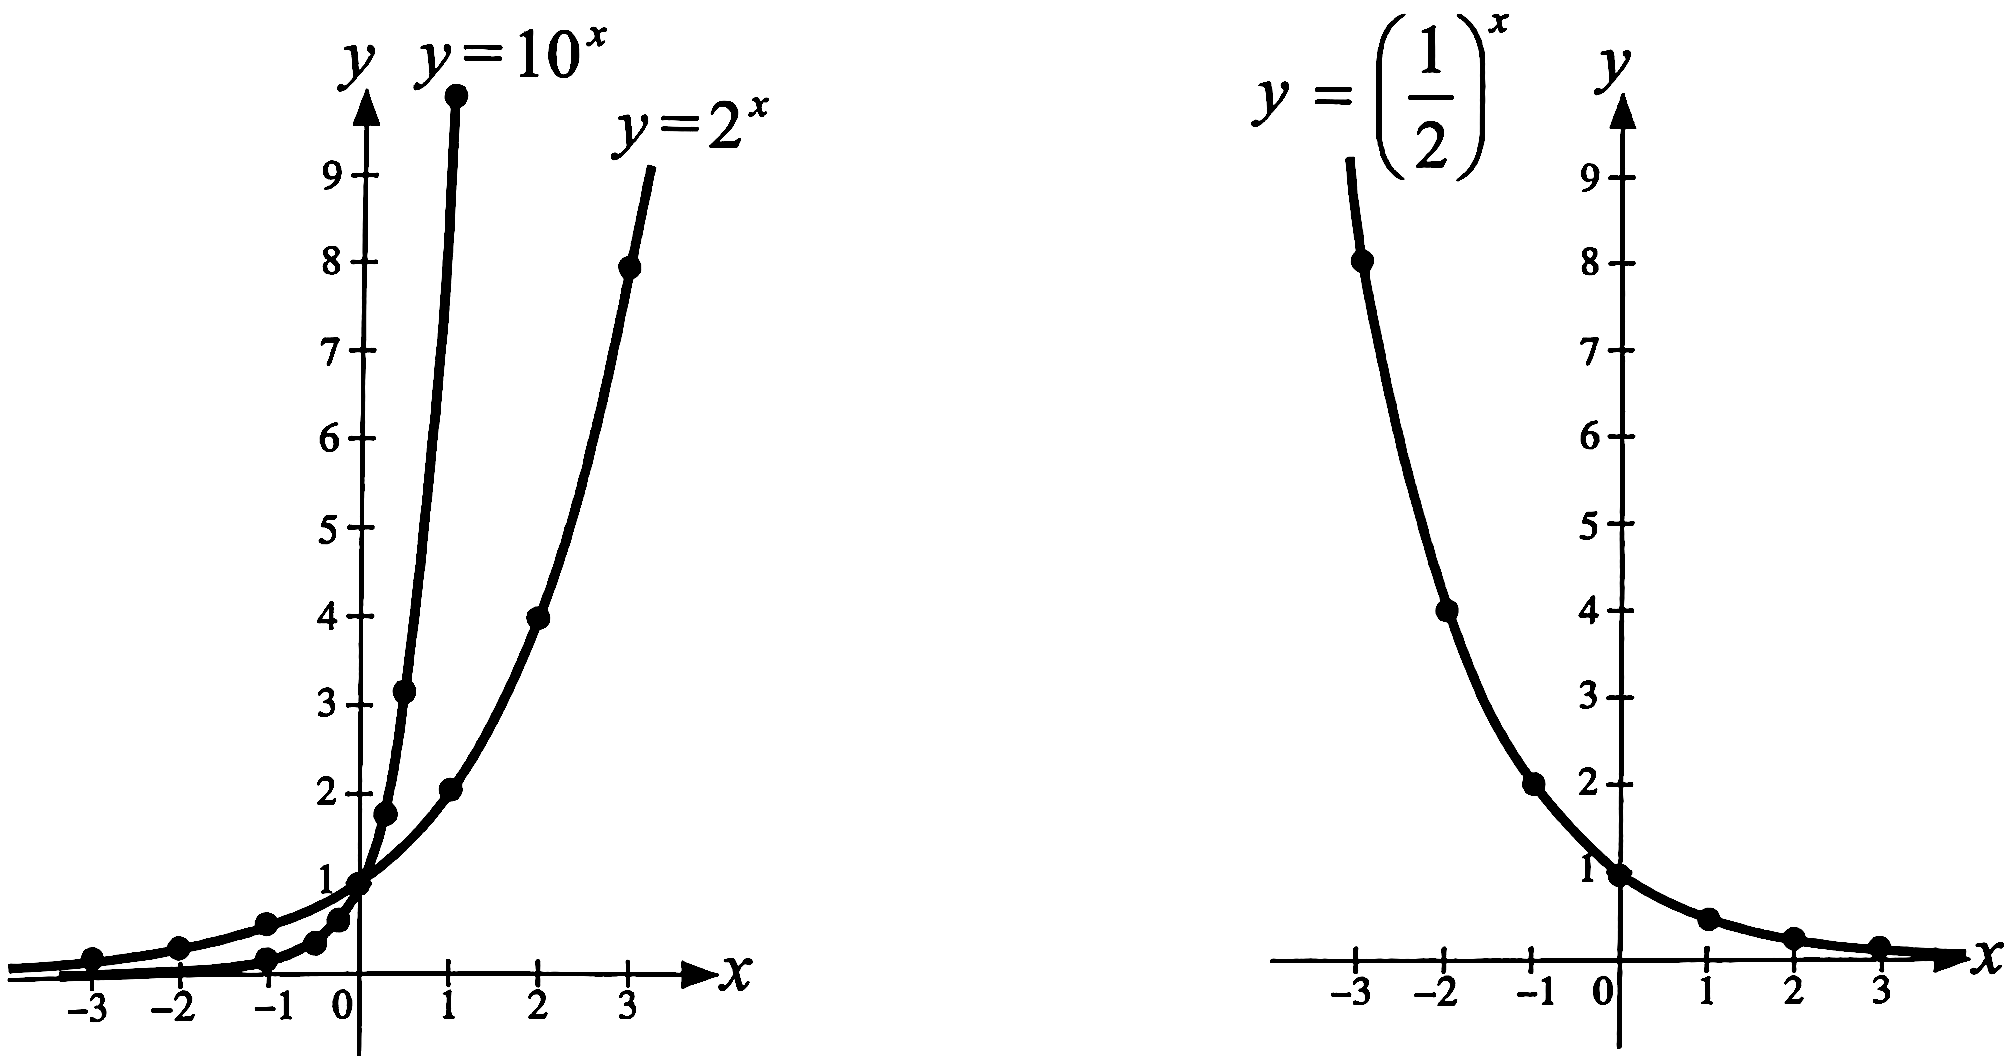
\includegraphics[width=0.6\textwidth]{assets/12-1.png}
    \end{center}

    \vspace{-1em}
    From the graphs, we can see that:

    \vspace{-1em}
    \begin{itemize}
        \item The graphs of the functions $y=2^x$, $y=10^x$, and $y=\left(\dfrac{1}{2}\right)^x$ are all located above the x-axis. In fact, since $a > 0$, then $a^x > 0$, the values of the exponential function $y=a^x$ are always greater than 0.
        \item The $ $-axis is the asymptote of the exponential function $y=a^x$.
        \item When $x=0$, $y=a^0=1$. Therefore, all the graphs of the exponential functions $y=a^x$ pass through the point $(0,1)$.
        \item For the functions $y=2^x$ and $y=10^x$, when $x>0$, $y>1$; when $x<0$, $0<y<1$. As the value of $x$ increases, the value of $y$ also increases, meaning the functions are increasing on the interval $(-\infty, \infty)$.
        \item For the function $y=\left(\dfrac{1}{2}\right)^x$, when $x>0$, $0<y<1$; when $x<0$, $y>1$. As the value of $x$ increases, the value of $y$ decreases, meaning the function is decreasing on the interval $(-\infty, \infty)$.
    \end{itemize}

    \vspace{-1em}
    Hence, when we are discussing the graphs and properties of the function $y=a^x$, we must discuss the cases where $a > 1$ and $0 < a < 1$ separately, as shown in the following table:

    \begin{center}
        \begin{NiceTabular}{*{3}{c}}[corners,hvlines]
            & $a > 1$ & $0 < a < 1$ \\
            Graph & 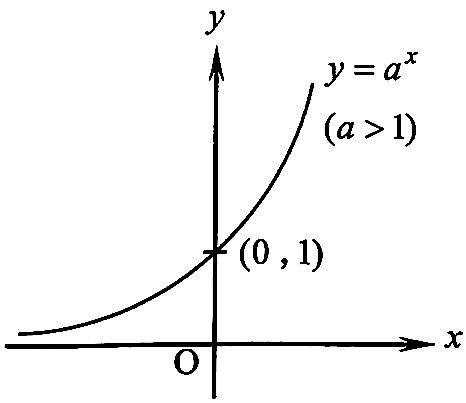
\includegraphics[scale=0.2]{assets/12-2.jpeg} & 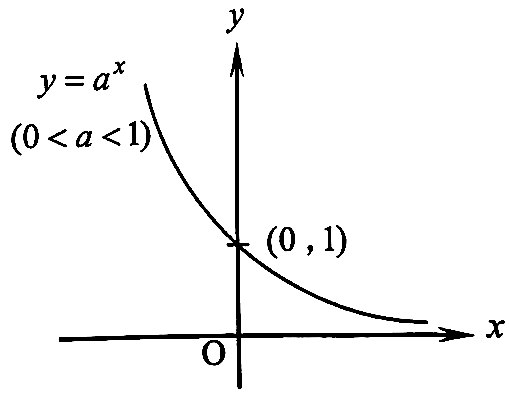
\includegraphics[scale=0.2]{assets/12-3.jpeg} \\
            \Block{4-1}{Properties} & \Block{1-2}{$y > 0$, i.e. range $= (0, \infty)$} \\
            & \Block{1-2}{When $x = 0$, $y = 1$} \\
            & \Block{}{When $x > 0$, $y > 1$;\\When $x < 0$, $0 < y < 1$} & \Block{}{When $x > 0$, $0 < y < 1$;\\When $x < 0$, $y > 1$} \\
            & \Block{}{It is an increasing function\\in the interval $(-\infty, +\infty)$} & \Block{}{It is a decreasing function\\in the interval $(-\infty, +\infty)$} \\
        \end{NiceTabular}
    \end{center}

    \begin{explore}[Exploration Activity 1]
        
        \textbf{Aim:} To explore the graph of the exponential function.
        
        \textbf{Tool:} \url{https://www.geogebra.org/m/rweqzcrt}
    \end{explore}
    \vspace{1em}

    \begin{question}
        Without using a calculator, compare the two values in each of the following pairs:
        \begin{tasks}[label=(\alph*)](3)
            \task $1.5^{3.1}$ and $1.5^{3.5}$
            \task $0.7^{2.3}$ and $0.7^{3.2}$
            \task $0.2^{-5.1}$ and $0.2^{-4.1}$
        \end{tasks}

        \sol{}
        \begin{tasks}[label=(\alph*)]
            \task Since the base number $1.5>1$, the exponential function $y=1.5^x$ is increasing in the interval $(-\infty, \infty)$,
            the exponent $3.1<3.5$
            
            $
            \therefore 1.5^{3.1}<1.5^{3.5}
            $

            \task Since the base number $0<0.7<1$, the exponential function $y=0.7^x$ is decreasing in the interval $(-\infty, \infty)$,
            the exponent $2.3<3.2$
            
            $
            \therefore 0.7^{2.3}>0.7^{3.2}
            $

            \task Since the base number $0<0.2<1$, the exponential function $y=0.2^x$ is decreasing in the interval $(-\infty, \infty)$,
            the exponent $-5.1<-4.1$

            $
            \therefore 0.2^{-5.1}>0.2^{-4.1}
            $
        \end{tasks}
    \end{question}
\vspace{-1em}
    \begin{question}
        Solve the inequality $\left(\dfrac{1}{2}\right)^x \leq\left(\dfrac{1}{2}\right)^{x^2}$.

        \sol{}
        \vspace{-2.5em}
        \begin{multicols}{2}
            \begin{flalign*} 
                & \left(\frac{1}{2}\right)^x \leq\left(\frac{1}{2}\right)^{x^2} &\\ 
                & \because y=\left(\frac{1}{2}\right)^x \text { is a decreasing function, }  
                \end{flalign*}
                \vspace{-3em}
                \begin{flalign*}
                    x &\geq x^2 &\\ 
                \quad x(x-1) &\leq 0
                \end{flalign*}
                \vspace{-3.5em}
                
                \noindent $\therefore 0 \leq x \leq 1$

                \begin{center}
                    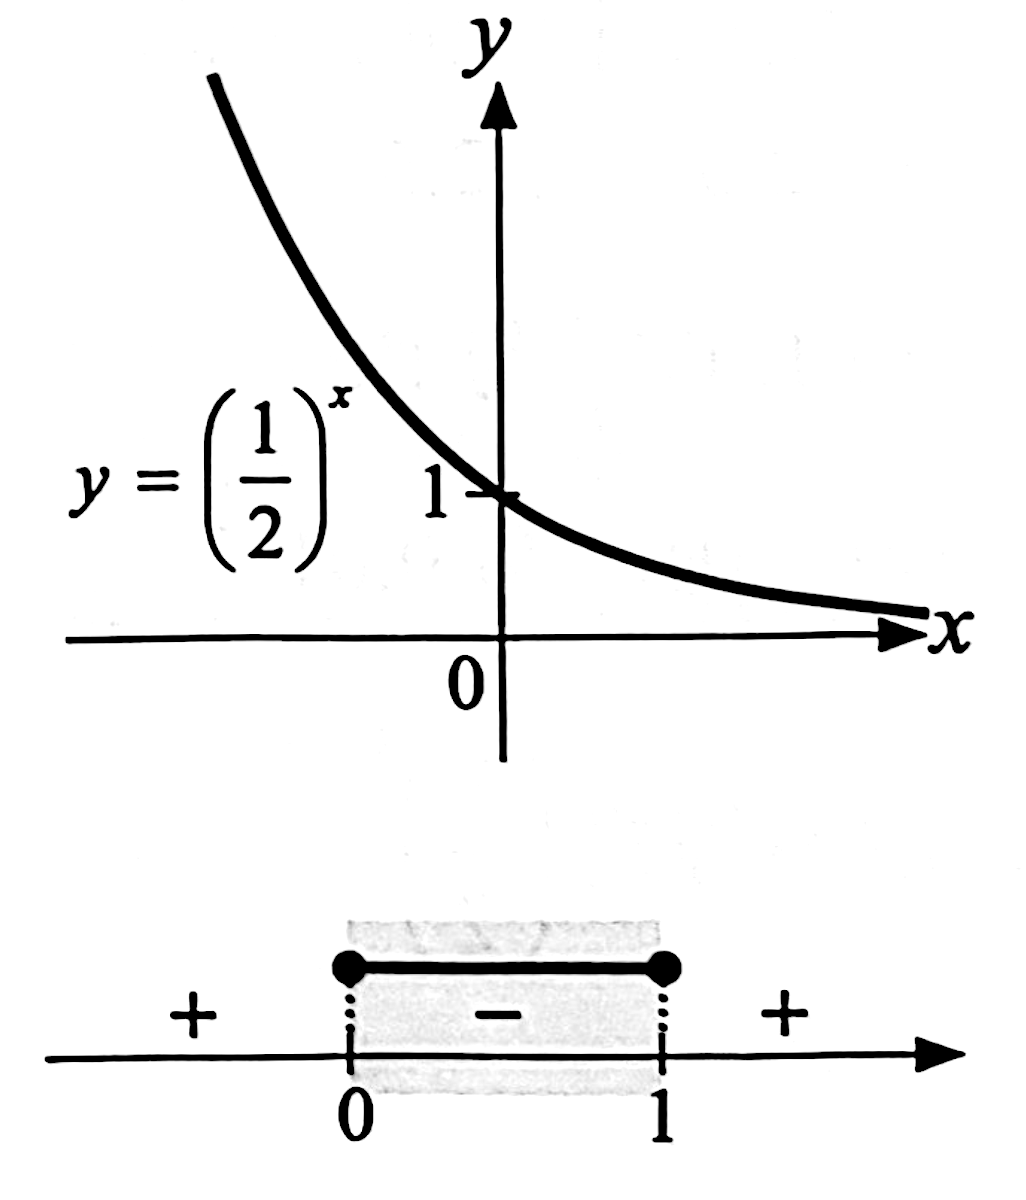
\includegraphics[width=0.25\textwidth]{assets/12-4.png}
                \end{center}
        \end{multicols}
        \vspace*{-3em}
    \end{question}
    \vspace{-2em}
    \practice{12.1b}
        \begin{enumerate}
            \item Without using a calculator, compare the two values in each of the following pairs:
            \begin{tasks}[label=(\alph*)](2)
                \task $\pi^{2.1}$ and $\pi^{3.5}$
                \task $0.15^{-2.3}$ and $0.15^{-3.8}$
            \end{tasks}
            \item Solve the inequality $3^{x^2-3 x+5} \geq 3^{x+10}$.
        \end{enumerate}

        \exercise{12.1}

        \noindent Calculate (Question 1 to 4):
        \begin{tasks}[label=\arabic*.](2)
            \task $\displaystyle\left(2 \frac{1}{4}\right)^{-\frac{3}{2}}+\left(1 \frac{11}{25}\right)^{-\frac{1}{2}}-\left(2 \frac{2}{3}\right)^0$
            \task $\displaystyle12^{\frac{1}{3}} \times 6^{\frac{1}{3}} \div 27^{\frac{1}{6}} \div 3^{\frac{1}{6}}$
            \task $\displaystyle\left(\frac{1}{2}\right)^{-2}+125^{\frac{2}{3}}+343^{\frac{1}{3}}-\left(\frac{1}{27}\right)^{-\frac{1}{3}}$
            \task $\displaystyle\frac{\sqrt[5]{4} \cdot \sqrt{8}(\sqrt[3]{\sqrt[5]{4}})^2}{\sqrt[3]{\sqrt{2}}}$
        \end{tasks}

        \vspace{-0.5em}
        \noindent Simplify the following expressions (Question 5 to 8):
        \begin{tasks}[label=\arabic*., start=5](2)
            \task $\displaystyle\left(\frac{b}{2 a^2}\right)^3 \div\left(\frac{2 b^2}{3 a}\right)^0 \times\left(-\frac{b}{a}\right)^{-3}$
            \task $\displaystyle\left(x^{\frac{1}{4}}-y^{-\frac{1}{4}}\right)\left(x^{\frac{1}{2}}+y^{-\frac{1}{2}}\right)\left(x^{\frac{1}{4}}+y^{-\frac{1}{4}}\right)$
            \task $\displaystyle\frac{3 \cdot 2^n-4 \cdot 2^{n-2}}{2^n-2^{n-1}}$
            \task $\displaystyle\frac{3^{n+6}-6 \cdot 3^{n+1}}{7 \cdot 3^{n+2}}$
        \end{tasks}

        \vspace{-1.5em}
        \begin{enumerate}[start=9]
            \item Given that $a^{2 x}=\sqrt{2}+1$, find the value of $\dfrac{a^{3 x}+a^{-3 x}}{a^x+a^{-x}}$.
            \item In the same Cartesian coordinates system, sketch the graphs for $y=3^x$ and $y=\left(\frac{1}{3}\right)^x$.
            \item Without using a calculator, compare the two values in each of the following pairs:
            \begin{tasks}[label=(\alph*)](2)
                \task $2.5^{7.1}$ and $2.5^{8.5}$
                \task $0.35^{6.5}$ and $0.35^{5.6}$
                \task $1.03^{-2.1}$ and $1.03^{-3.2}$
                \task $(\sqrt{2})^\pi$ and $(\sqrt{2})^{3.5}$
                \task $0.01^{-\frac{1}{3}}$ and $0.01^{-\frac{1}{2}}$
                \task $2.7^{\sqrt{20}}$ and $2.7^{\sqrt[3]{35}}$
            \end{tasks}
            \item Solve the inequality $\left(\dfrac{1}{2}\right)^{3 x-x^2}<1$.
        \end{enumerate}
        
        \section{Logarithms}

        \subsection*{Definition of Logarithms and its Properties}

        Let $a$ be a positive integer and $a \neq 1$. If $a^n = x$, then we define $\log_a x = n$, read as ``logarithm of $x$ to the base $a$ is $n$''. In $\log_a x = n$, $a$ is called the \textbf{base}, and $x$ is called the \textbf{antilogarithm}.

        Conversely, if $\log_a x = n$, then $a^n = x$. That is,
        \begin{info}[Definition of Logarithms]
           $$a^n = x \iff \log_a x = n \qquad\text{where $a > 0, a \neq 1$, $x > 0$}$$
        \end{info}

        From this, we can get
        \begin{info}[Properties of Logarithms]
            $$\log_a a^n = n$$
        \end{info}
            
        \newpage
        When $n = 1$ and $n = 0$, we have the following special cases:
        \begin{info}[Special Cases of Logarithms]
            \begin{flalign*}
                \log_a a &= 1 &\\
                \log_a 1 &= 0 &
            \end{flalign*}
        \end{info}

        The logarithm with base 10 is called the \textbf{common logarithm}, denoted as $\log_{10} x$, $\log x$, or $\lg x$. 
        
        There also exists a special base $e$ in logarithms. It is an irrational number approximately equal to 2.71828. The logarithm with base $e$ is called the \textbf{natural logarithm}, denoted as $\log_e x$, $\ln x$. It is widely used in the fields of natural science.

        \begin{question}
            If $\log_3 x = 5$, find the value of $x$.

            \sol{}
            \begin{flalign*}
                \log_3 x &= 5 &\\
                x &= 3^5 &\\
                &= 243 &
            \end{flalign*}
        \end{question}

        \begin{question}
            Find the value of the following:
            \begin{tasks}[label=(\alph*)](2)
                \task $\log _5 5$
                \task $\lg 1$
                \task $\log _7 343$
                \task $\ln \frac{1}{e^2}$
            \end{tasks}

            \sol{}
            \begin{tasks}[label=(\alph*)](2)
                \task $\log _5 5=1$
                \task $\lg 1=0$
                \task $\log _7 343=\log _7 7^3=3$
                \task $\ln \dfrac{1}{e^2}=\ln e^{-2}=-2$
            \end{tasks}
        \end{question}

        \practice{12.2a}
        \begin{enumerate}
            \item If $\log_4 x = -2$, find the value of $x$.
            \item Find the value of the following:
            \begin{tasks}[label=(\alph*)](2)
                \task $\log_2 \dfrac{1}{2}$
                \task $\lg 10$
                \task $\log_\frac{1}{3} 27$
                \task $\log_4 \dfrac{1}{128}$
            \end{tasks}
        \end{enumerate}

        \subsection*{Arithmetic Rules of Logarithms}

        If $a$, $x$, and $y$ are positive numbers, and $x = a^p$, $y = a^q$, then $\log_a x = p$ and $\log_a y = q$. 
        
        \begin{itemize}
            \item $\begin{aligned}[t] x y & =a^p \times a^q=a^{p+q} \\ \therefore \log _a(x y) & =p+q \\ & =\log _a x+\log _a y\end{aligned}$
            \item $\begin{aligned}[t] \frac{x}{y} & =a^p \div a^q=a^{p-q} \\ \therefore \log _a \frac{x}{y} & =p-q \\ & =\log _a x-\log _a y\end{aligned}$
            \item $x=a^p\ \cdots\ (1)$, then $\log _a x=p\ \cdots\ (2)$
            
            Substituting $(2)$ into $(1)$, we get $x=a^{\log _a x}$
        \end{itemize}

        Summarizing the above, we have the following properties of logarithms:
        \begin{info}[Arithmetic Properties of Logarithms]
            If $x > 0$, $y > 0$,
            \begin{flalign*}
                \log _a(x y) &= \log _a x+\log _a y &\\
                \log _a\frac{x}{y} &= \log _a x-\log _a y &\\
                \log _a x^m &= m \log _a x &\\
                a^{\log _a x} &= x &
            \end{flalign*}
        \end{info}
        
        \begin{question}
            Let $a = \log_2$, express the following in terms of $a$:
            \begin{tasks}[label=(\alph*)](2)
                \task $\log 8^2$
                \task $\left(\log 8\right)^2$
            \end{tasks}

            \sol{}
            \begin{tasks}[label=(\alph*)](2)
                \task $\begin{aligned}[t]
                    \log 8^2 &= \log 2^6 \\
                    &= 6 \log 2 \\
                    &= 6 a
                \end{aligned}$
                \task $\begin{aligned}[t]
                    \left(\log 8\right)^2 &= \left(\log 2^3\right)^2 \\
                    &= \left(3 \log 2\right)^2 \\
                    & = (3a)^2\\
                    &= 9 a^2
                \end{aligned}$
            \end{tasks}
        \end{question}

        \newpage
        \begin{question}
            Without using a calculator, find the value of the following:
            \begin{tasks}[label=(\alph*)](2)
                \task $100^{\log 3}$
                \task $2 \log _3 15-\log _3 50+\log _3 6$
            \end{tasks}

            \sol{}
            \begin{tasks}[label=(\alph*)]
                \task $\begin{aligned}[t]
                    100^{\log 3} & =10^{2 \log 3} \\
                    & =10^{\log 3^2} \\
                    & =9
                \end{aligned}$
                \task $\begin{aligned}[t]
                    2 \log _3 15-\log _3 50+\log _3 6 & =\log _3(15)^2-\log _3 50+\log _3 6 \\
                    & =\log _3 \frac{225 \times 6}{50} \\
                    & =\log _3 3^3 \\
                    & =3
                \end{aligned}$
            \end{tasks}
        \end{question}

        \begin{question}
            Given that $\log_2 3 = a$, $\log_2 5 = b$. Express the following in terms of $a$ and $b$:
            \begin{tasks}[label=(\alph*)](2)
                \task $\log _2 30$
                \task $\log _2 \sqrt{1.25}$
            \end{tasks}

            \sol{}
            \begin{tasks}[label=(\alph*)]
                \task
                $
                \begin{aligned}[t]
                \log _2 30 & =\log _2(2 \times 3 \times 5) \\
                & =\log _2 2+\log _2 3+\log _2 5 \\
                & =1+a+b
                \end{aligned}
                $
                \task
                $
                \begin{aligned}[t]
                \log _2 \sqrt{1.25} & =\log _2\left(\frac{5}{4}\right)^{\frac{1}{2}} \\
                & =\frac{1}{2}\left(\log _2 5-\log _2 2^2\right) \\
                & =\frac{1}{2}(b-2)
                \end{aligned}
                $
            \end{tasks}
        \end{question}

        \practice{12.2b}
        \begin{enumerate}
            \item Calculate the following:
            \begin{tasks}[label=(\alph*)](2)
                \task $2^{\log _2 7}$
                \task $\log \dfrac{1}{35}+\log 70-\log \dfrac{1}{2}+2 \log 5$
            \end{tasks}

            \item Given that $\log_3 2 = a$, $\log_3 5 = b$, express $\log_3 3.75$ in terms of $a$ and $b$.
        \end{enumerate}

        \subsection*{Change of Base Formula}

        Some commonly used calculator calculate logarithms using base 10 or $e$. The change of base formula allows for the conversion of logarithms with any base to those with base 10 or $e$, making it easy to calculate logarithms with bases other than 1.
        
        The change of base formula also facilitates simplification of computations by converting logarithms with different bases to those with the same base.

        If $\log_a b = n$, then
        
        $\begin{aligned} a^n & =b \\ \log _c a^n & =\log _c b \\ n \log _c a & =\log _c b \\ n & =\frac{\log _c b}{\log _c a}\end{aligned}$

        \begin{info}[Change of Base Formula]
            $$\log _a b=\frac{\log _c b}{\log _c a}$$
        \end{info}

        Using the change of base formula, we can convert logarithms with any base to a specific base. In the formula, let $c = b$, we get
        \begin{info}[Change of Base Formula (Special Case)]
            $$\log _a b=\frac{1}{\log _b a}$$
        \end{info}

        \begin{question}
            Find the value of $\log_3 5$.

            \sol{}
            \begin{flalign*}
                \log_3 5 &= \frac{\log_{10} 5}{\log_{10} 3} = 1.4650 &
            \end{flalign*}
        \end{question}

        \begin{question}
            Without using a calculator, find the value of the following:
            \begin{tasks}[label=(\alph*)](2)
                \task $\log_8 32$
                \task $\log_{\sqrt{3}} \dfrac{1}{81}$
            \end{tasks}

            \sol{}
            \begin{tasks}[label=(\alph*)](2)
                \task $\begin{aligned}[t]
                    \log _8 32 &=\frac{\log _2 2^5}{\log _2 2^3} =\frac{5}{3}
                \end{aligned}$

                \task $
                \begin{aligned}[t]
                \log _{\sqrt{3}} \frac{1}{81} & =\frac{\log _3 3^{-4}}{\log _3 3^{\frac{1}{2}}} =\frac{-4}{\frac{1}{2}} =-8
                \end{aligned}
                $
                
            \end{tasks}
        \end{question}

        \begin{think}
            
            In Example 11, can they be changed into logarithms with other bases?
        \end{think}

        \vspace{1em}

        \begin{question}
            Given that $\log_2 3 = x$, $\log_3 5 = y$, express $\log_9 2.5$ in terms of $x$ and $y$.

            \sol{}
            \begin{flalign*}
                \log _9 2.5 & =\frac{\log _3 \frac{5}{2}}{\log _3 3^2} \\ & =\frac{\log _3 5-\log _3 2}{2} \\ & =\frac{1}{2}\left(y-\frac{1}{\log _2 3}\right) \\ & =\frac{1}{2}\left(y-\frac{1}{x}\right) \\ & =\frac{x y-1}{2 x} &
            \end{flalign*}
        \end{question}

        \practice{12.2c}

        \begin{enumerate}
            \item Without using a calculator, find the value of $\dfrac{\log_4 27}{\log_2 3}$.
            \item If $\log_2 3 = a$, $\log_5 3 = b$, express $\log 5$ in terms of $a$ and $b$.
        \end{enumerate}

        \begin{question}
            Given that $3 \log _7\left(x y^2\right)+\log _7 x=4+2 \log _7 y$, express $y$ in terms of $x$.

            \sol{}
            \begin{flalign*}
                3 \log _7\left(x y^2\right)+\log _7 x & =4+2 \log _7 y \\
                3\left(\log _7 x+\log _7 y^2\right)+\log _7 x-2 \log _7 y & =4 \\
                4 \log _7 x+4 \log _7 y & =4 \\
                \log _7 x+\log _7 y & =1 \\
                \log _7(x y) & =1 \\
                x y & =7 &\\
                y & =\frac{7}{x}
                \end{flalign*}
        \end{question}

        \exercise{12.2a}

        Find the value of $x$ in the following (Question 1 to 2):
        \begin{tasks}[label=\arabic*.](2)
            \task $\log _{125} x=\dfrac{1}{3}$
            \task $\log _x 81=-4$
        \end{tasks}

        \noindent Simplify the following expressions (Question 3 to 8):
        \begin{tasks}[label=\arabic*., start=3](2)
            \task $\log _2 4^x$
            \task $\log _2 a^{\log _a 2}$
            \task $3^{\log _3 x-\log _3 y}$
            \task $\log _3\left(9^x \times 27^y\right)$
            \task $2^{-\log _8 x}$
            \task $3 \log _4 2^x$
        \end{tasks}

        \noindent Without using a calculator, find the value of the following (Question 9 to 18):
        \begin{tasks}[label=\arabic*., start=9](2)
            \task $\displaystyle\log _7 \sqrt[3]{49}$
            \task $\displaystyle49^{\log _7 3}$
            \task $\displaystyle\left(\frac{1}{2}\right)^{\log _2 7}$
            \task $\displaystyle\frac{\log \sqrt{3}}{\log \frac{1}{9}}$
            \task $\displaystyle\log (0.1)^4-\log \sqrt[3]{0.001}$
            \task $\displaystyle\frac{\log 4+\log 3}{1+\log 0.4+\frac{1}{2} \log 9}$
            \task $\displaystyle\log _2 \frac{1}{25} \cdot \log _3 \frac{1}{8} \cdot \log _5 \frac{1}{9}$
            \task $\displaystyle\log _4 5 \cdot \log _5 6 \cdot \log _6 7 \cdot \log _7 8$
            \task $\displaystyle\left(\log _2 3+\log _2 \sqrt{3}\right) \log _{\sqrt{3}} 2$
            \task $\displaystyle\frac{1}{2} \log \frac{81}{17}+2 \log \frac{5}{3}-\log \frac{17}{4}+\frac{3}{2} \log 17$
        \end{tasks}
        \begin{tasks}[label=\arabic*, resume]
            \task Given that $\log _2 3=a$ and $\log _2 5=b$. Express $\log _4 15$ in terms of $a$ and $b$.
            \task Given that $\log _3 5=m$ and $\log _5 6=n$. Express $\log _{25} 54$ in terms of $m$ and $n$.
            \task Given that $2^a=3$ and $3^b=7$. Express $\log _{42} 14$ in terms of $a$ and $b$.
            \task Given that $\log _3 6=x$. Express $\log _9 12$ in terms of $x$.
            \task If $\log 24=a$ and $\log 18=b$, express $\log 1.35$ in terms of $a$ and $b$.
            \task Given that $\log _{25}(2 x-1)=\log _5(x-3)+\log _{25} 5$, prove $5 x^2-32 x+46=0$.
            \task If $a, b, x$ are positive numbers, and $a, b$ are not equal to 1, prove $\displaystyle\frac{1}{\log _a x}+\frac{1}{\log _b x}=\frac{1}{\log _{a b} x}$.
        \end{tasks}

        \subsection*{Graph of Logarithmic Functions and its Properties}

        According to the definition of logarithms, if $y=2^x$, then $x=\log _2 y$. Because $y=2^x$ is a one-to-one function mapping from the set of real numbers to the set of positive real numbers, it has an inverse function. According to the concept of inverse functions, $y=\log _2 x$ is the inverse function of $y=2^x$. The function $y=\log _a x$ is called a \textbf{logarithmic function}, where $a>0$ and $a \neq 1$. Since the domain of the exponential function $y=a^x$ is the set of real numbers and the range is the set of positive real numbers, the domain of the logarithmic function $y=\log _a x$ is the set of positive real numbers, and the range is the set of real numbers.

        Since the logarithmic function $y=\log _a x$ is the inverse function of the exponential function $y=a^x$, the graph of $y=\log _a x$ is symmetric to the graph of $y=a^x$ about the line $y=x$. We only need to draw the curve symmetric to the graph of $y=a^x$ about the line $y=x$ to obtain the graph of $y=\log _a x$. For example, in the figures below, the curves symmetric to the graph of the functions $y=2^x$ and $y=\left(\frac{1}{2}\right)^x$ about the line $y=x$ are the graphs of $y=\log _2 x$ and $y=\log _{\frac{1}{2}} x$, respectively.
        \begin{center}
            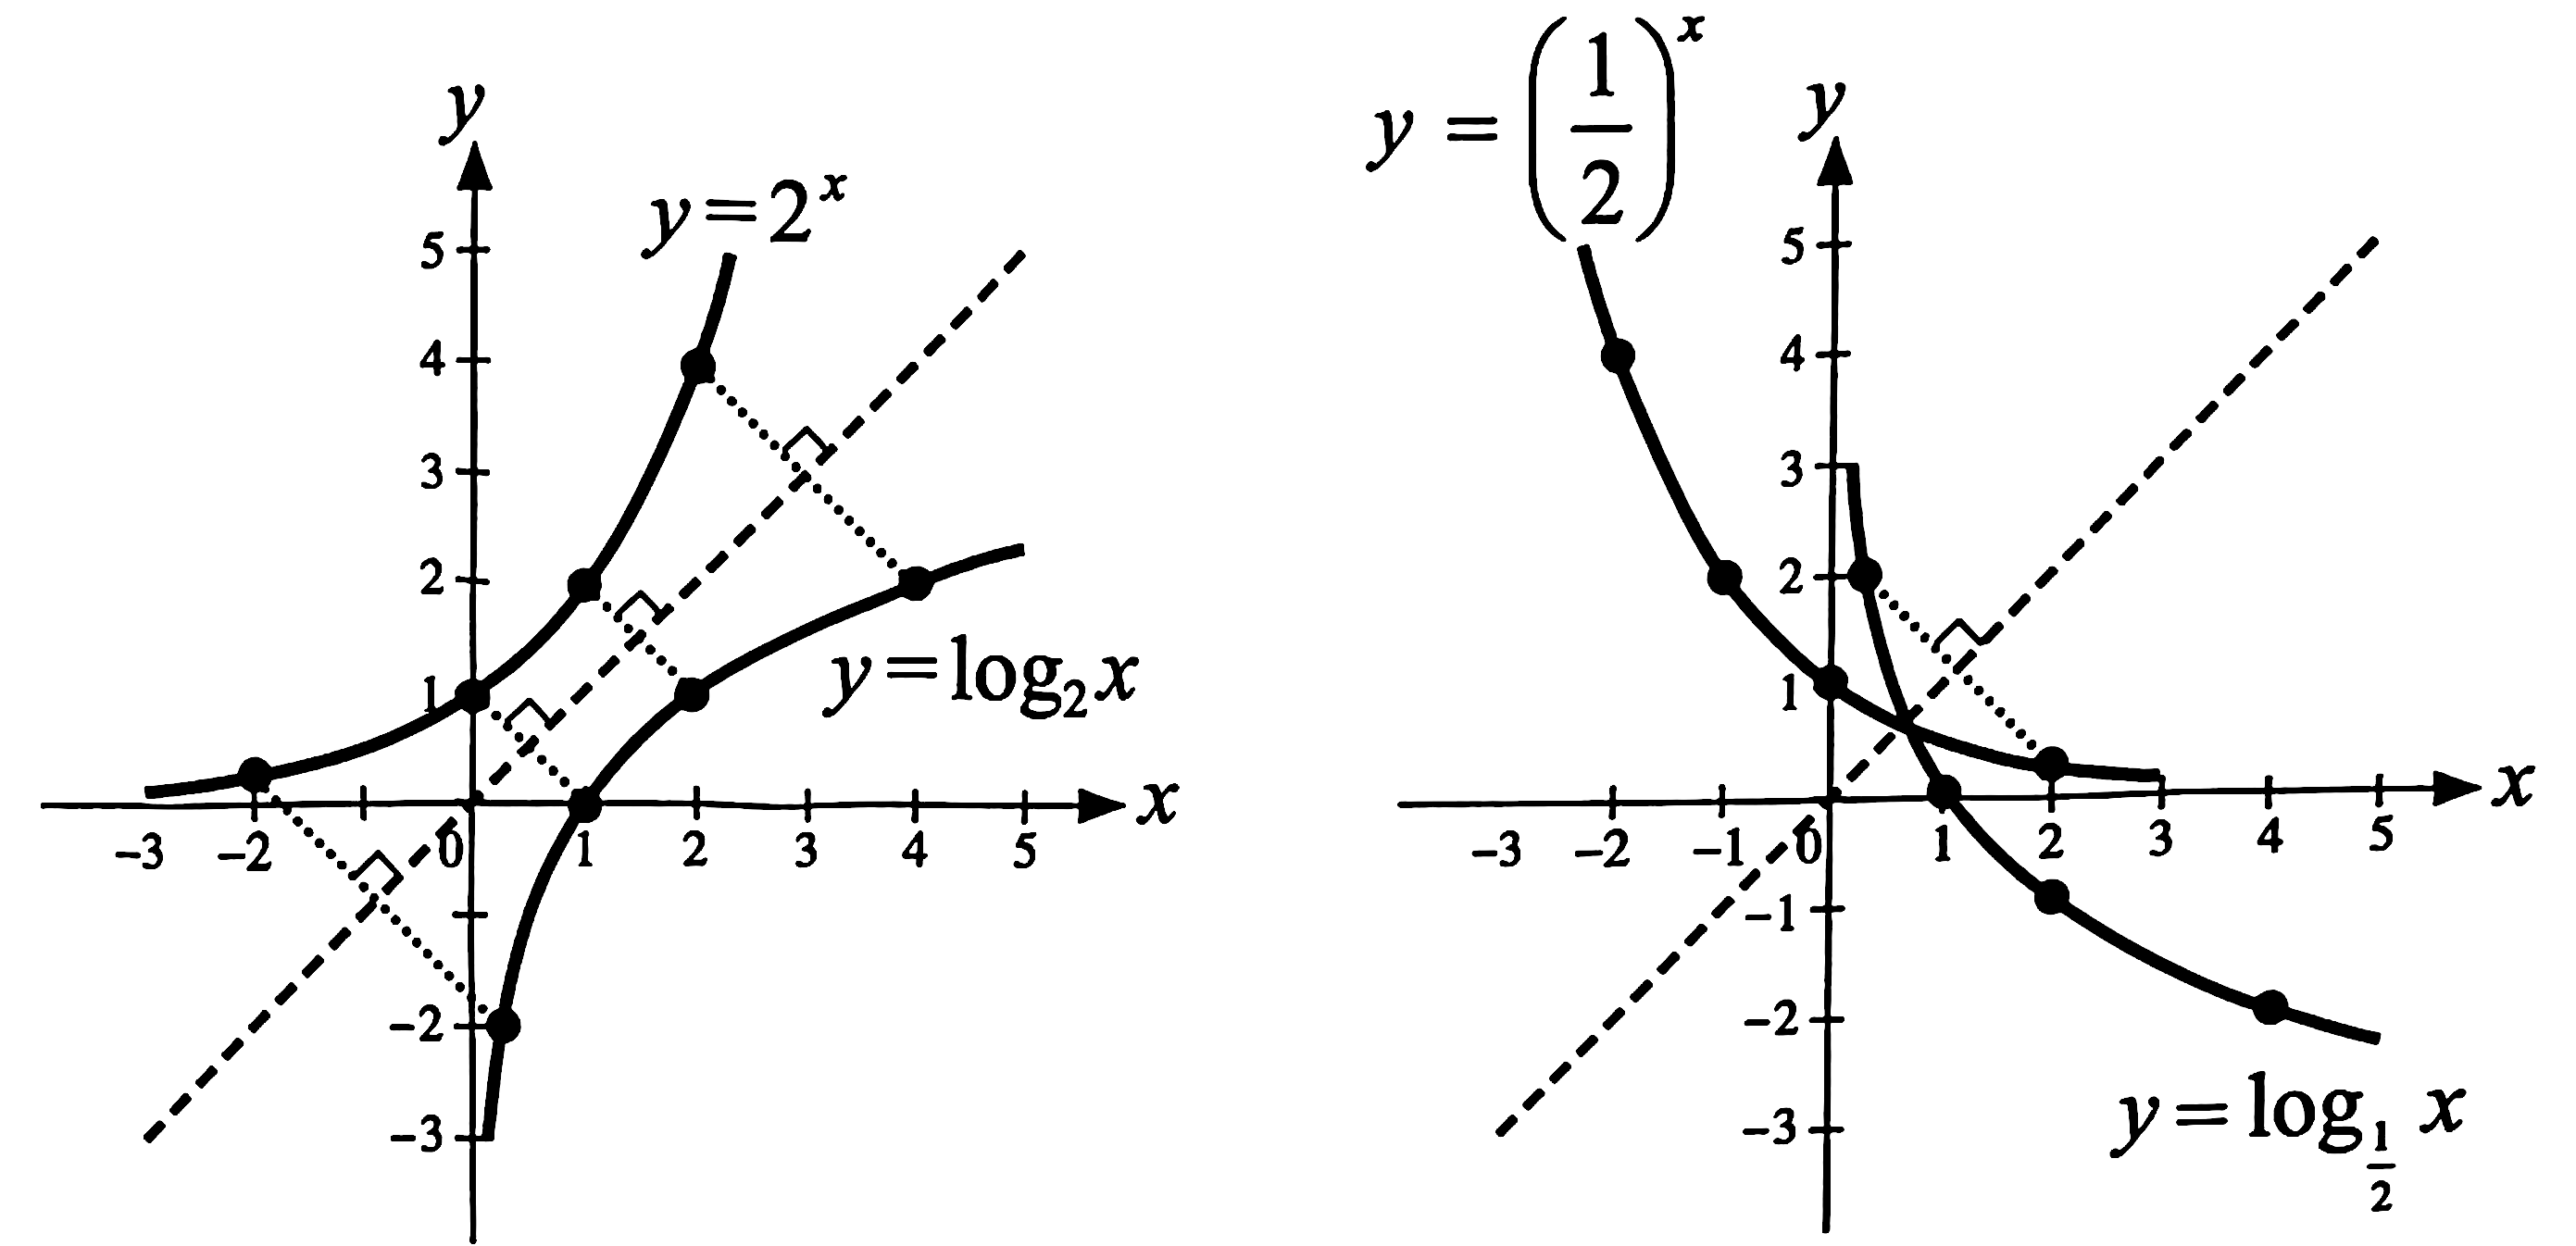
\includegraphics[width=0.6\textwidth]{assets/12-5.png}
        \end{center}

        From the graphs, we can see that:
        \begin{itemize}
            \item The graphs of the functions $y=\log _2 x$ and $y=\log _{\frac{1}{2}} x$ are located only to the right of the $y$-axis because their domains are $(0, \infty)$.
            The $y$-axis serves as the asymptote for the logarithmic function $y=\log _a x$.
            \item When $x=1$, $y=\log _a 1=0$, so the graphs of the logarithmic functions $y=\log _a x$ all pass through the point $(1,0)$.
            \item For the function $y=\log _2 x$, when $x>1$, $y>0$; when $0<x<1$, $y<0$. As the value of $x$ increases, the value of $y$ also increases, meaning the function is increasing over the interval $(0, \infty)$.
            \item For the function $y=\log _{\frac{1}{2}} x$, when $x>1$, $y<0$; when $0<x<1$, $y>0$. As the value of $x$ increases, the value of $y$ decreases, indicating the function is decreasing over the interval $(0, \infty)$.
        \end{itemize}

        From the above, we can see that when discussing the graphs and properties of the function $y=\log _a x$, we must discuss the cases where $a > 1$ and $0 < a < 1$ separately, as shown in the following table:

        \begin{center}
            \begin{NiceTabular}{*{3}{c}}[corners,hvlines]
                & $a > 1$ & $0 < a < 1$ \\
                \Block{}{Graph} & 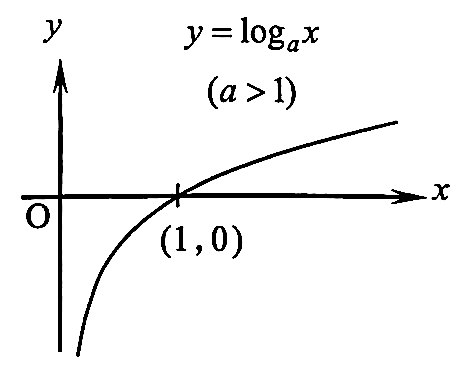
\includegraphics[scale=0.2]{assets/12-6.jpg} & 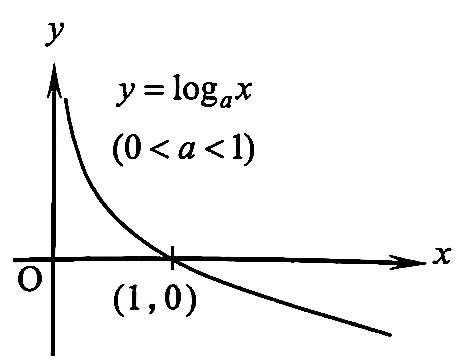
\includegraphics[scale=0.2]{assets/12-7.jpg} \\
                \Block{4-1}{Properties} & \Block{1-2}{$x > 0$, i.e. domain $= (0, \infty)$} \\
                & \Block{1-2}{When $x = 1$, $y = 0$} \\
                & \Block{}{When $x > 1$, $y > 0$;\\When $0 < y < 1$, $y < 0$} & \Block{}{When $x > 1$, $y < 0$;\\When $0 < x < 1$, $y > 0$} \\
                & \Block{}{It is an increasing function in \\the interval $(0, +\infty)$} & \Block{}{It is a decreasing function \\in the interval $(0, +\infty)$} \\
            \end{NiceTabular}
        \end{center}

        \begin{explore}[Exploration Activity 2]
            
            \textbf{Aim:} To explore the graph of the logarithmic function.
            
            \textbf{Tool:} \url{https://www.geogebra.org/m/ks3qqrua}
        \end{explore}

        \begin{question}
            Without using a calculator, compare the two values in each of the following pairs:
            \begin{tasks}[label=(\alph*)](2)
                \task $\log _3 5$ and $\log _3 7$
                \task $\log _{\frac{1}{2}} 5$ and $\log _{\frac{1}{2}} 9$
            \end{tasks}

            \sol{}
            \begin{tasks}[label=(\alph*)]
                \task Since the base $3 > 1$, the logarithmic function $y=\log_3 x$ is an increasing function in the interval $(0, \infty)$, the antilogarithm $5<7$

                $\therefore \log _3 5<\log _3 7$

                \task Since the base $0<\dfrac{1}{2}<1$, the logarithmic function $y=\log_{\frac{1}{2}} x$ is a decreasing function in the interval $(0, \infty)$, the antilogarithm $5<9$

                $\therefore \log _{\frac{1}{2}} 5>\log _{\frac{1}{2}} 9$
            \end{tasks}
        \end{question}

        \begin{question}
            Find the domain of the following functions:
            \begin{tasks}[label=(\alph*)](2)
                \task $f(x)=\log _a(x-4)$
                \task $y=\log _2\left(x^2+5\right)$
                \task $y=\log _3 \dfrac{x+3}{2-x}$
                \task $f(x)=\sqrt{\log _{\frac{1}{2}}(3-x)}$
            \end{tasks}

            \sol{}
            \begin{tasks}[label=(\alph*)]
                \task From $x-4>0$, we get $x>4$. 
                
                $\therefore$ the domain of the function $f(x)=\log _a(x-4)$ is ${x \mid x \in \mathbb{R}, x>4}$.

                \task For all $x \in \mathbb{R}$, $x^2+5>0$. 
                
                $\therefore$ the domain of the function $y=\log _2\left(x^2+5\right)$ is $\mathbb{R}$.
                
                \task From $2-x \neq 0$ and $\dfrac{x+3}{2-x}>0$, i.e. $\dfrac{x+3}{x-2}<0$, we get $-3<x<2$. 
                
                $\therefore$ the domain of the function $y=\log _3 \dfrac{x+3}{2-x}$ is ${x \mid x \in \mathbb{R}, -3<x<2}$.
                
                \task $x$ must satisfy both $3-x>0$ and $\log _{\frac{1}{2}}(3-x) \geq 0$, 
                
                i.e. $\left\{\begin{array}{c}x<3 \\ 3-x \leq 1\end{array} \Rightarrow 2 \leq x<3\right.$. 
                
                $\therefore$ the domain of the function $f(x)=\sqrt{\log _{\frac{1}{2}}(x-3)}$ is $[2,3)$.
            \end{tasks}
        \end{question}

        \begin{question}
            Solve the inequality $\log _{\frac{1}{3}}(2 x-1)+2>0$.

            \sol{}
            \vspace{-3em}
            \begin{multicols}{2}
                \begin{flalign*}
                    \log _{\frac{1}{3}}(2 x-1)+2&>0 &\\
                    \log _{\frac{1}{3}}(2 x-1)&>-2
                \end{flalign*}
                From the graph of $y = \log_{\frac{1}{3}} x$, we get:
                \begin{flalign*}
                    & 0<2 x-1<\left(\frac{1}{3}\right)^{-2} &\\
                    & 0<2 x-1<9
                \end{flalign*}
                $\therefore \dfrac{1}{2}<x<5$

                \columnbreak

                \vspace*{3em}

                \begin{center}
                    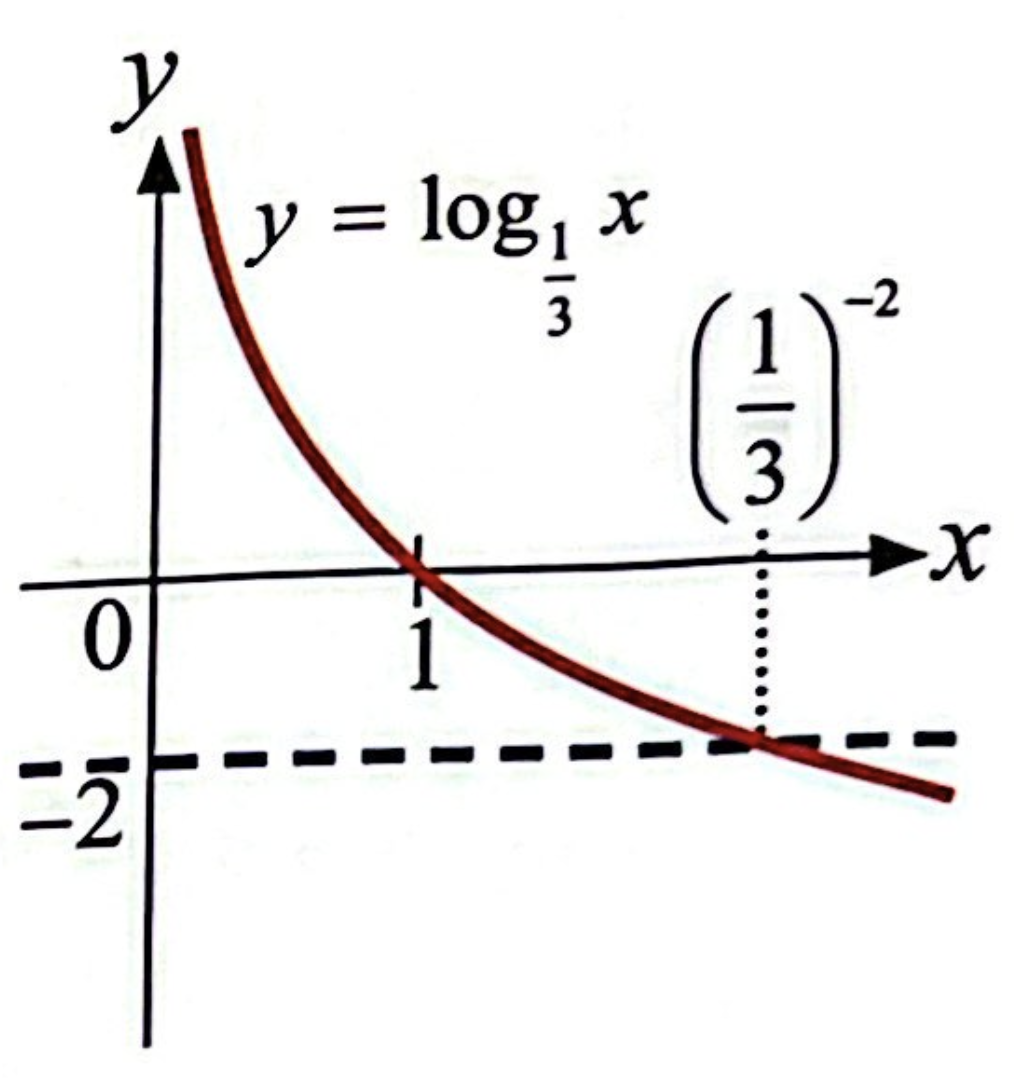
\includegraphics[width=0.2\textwidth]{assets/12-8.png}
                \end{center}
            \end{multicols}
        \end{question}
        \begin{question}
            Solve the inequality $\log _3\left(x^2-2 x\right)<1$.

            \sol{}
            \vspace{-1em}
            \begin{multicols}{2}
                \noindent $\log _3\left(x^2-2 x\right)<1$
            
            \noindent From the graph of $y = \log_3 x$, we know that $0 < x^2-2 x < 3$.

            \noindent Hence, we get the following system of inequalities:
            
            \noindent $\left\{\begin{array}{l}
                x^2-2 x>0\ \cdots\ (1) \\
                x^2-2 x<3\ \cdots\ (2)
                \end{array}\right.$

                \noindent From (1), we get $\begin{aligned}[t]
                    x(x-2)&>0 \\
                    x<0 \text { or } &x>2
                    \end{aligned}$

                \noindent From (2), we get $\begin{aligned}[t]
                    (x+1)(x-3)&<0 \\
                    -1<x<3
                    \end{aligned}$

                \noindent $\therefore$ the solution to the inequality $\log _3\left(x^2-2 x\right)<1$ is $-1<x<0$ or $2<x<3$.

                \columnbreak

                \vspace*{3em}

                \begin{center}
                    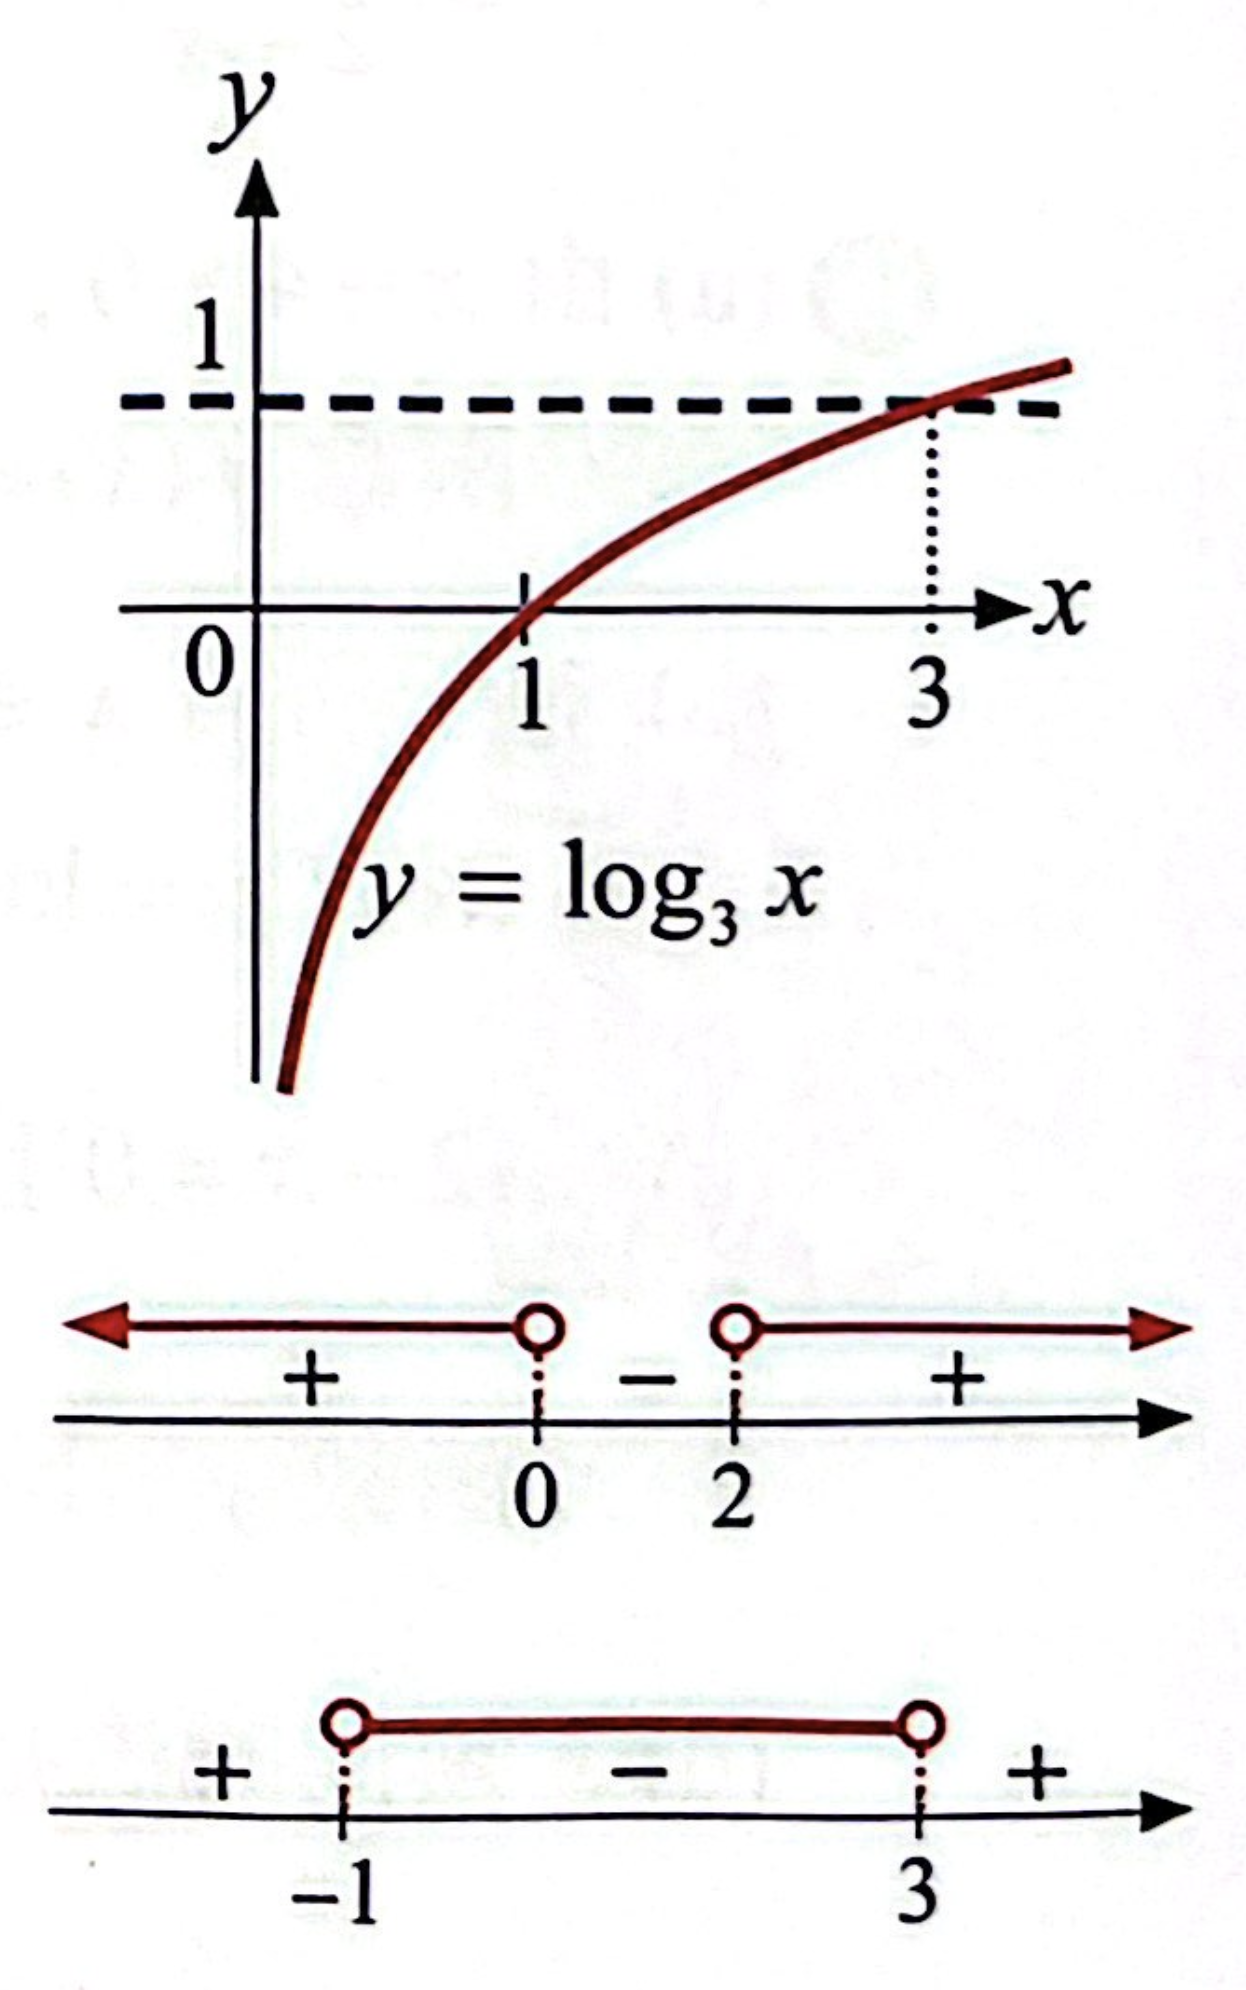
\includegraphics[width=0.25\textwidth]{assets/12-9.png}
                \end{center}
            \end{multicols}
        \end{question}

        \newpage
        \practice{12.2d}
        \begin{enumerate}
            \item Without using a calculator, compare the two values in each of the following pairs:
            \begin{tasks}[label=(\alph*)](2)
                \task $\log _{0.3} 5$ and $\log _{0.3} 7$
                \task $\log _{\frac{1}{2}} 0.4$ and $\log _2 0.7$
            \end{tasks}
            \item Find the domain of the following functions:
            \begin{tasks}[label=(\alph*)](2)
                \task $f(x)=\log _2\left(x^2+8\right)$
                \task $f(x)=\log _3 \dfrac{1-2 x}{x+2}$
            \end{tasks}
            \item Solve the inequality $\log _3\left(x^2-2 x\right) \geq 1$.
        \end{enumerate}

        \subsection*{Applications of Logarithms}

        \begin{question}
            In 1935, American scientist C. F. Richter proposed the Richter scale for measuring the magnitude of earthquakes, which is commonly denoted as \( M \), with the calculation formula \( M = \log_{10} A - \log_{10} A_0 \), where \( A \) is the maximum amplitude of the earthquake and \( A_0 \) is the amplitude of a "standard earthquake."
            \begin{tasks}[label=(\alph*)]
                \task Suppose in an earthquake, a seismometer located \( 100 \, \text{km} \) from the epicenter records a maximum amplitude of \( 30 \, \text{mm} \), and the amplitude of the standard earthquake (\( A_0 \)) is \( 0.001 \, \text{mm} \). Calculate the magnitude of this earthquake (accurate to \( 0.1 \)).

                \task How many times greater is the maximum amplitude of a 7.2 magnitude earthquake compared to that of a 5 magnitude earthquake?
            \end{tasks}

            \sol{}
            \begin{tasks}[label=(\alph*)]
                \task Magnitude $\begin{aligned}[t]
                    M & =\lg 30-\lg 0.001 \\
                    & =\lg \frac{30}{0.001} \\
                    & =\lg 30000 \\
                    & =4.5
                    \end{aligned}$

                    \task Since $M = \lg A - \lg A_0$, we get $\begin{aligned}[t]
                        M&=\lg \frac{A}{A_0} \\
                        \frac{A}{A_0}&=10^M \\
                        A&=A_0 \times 10^M
                        \end{aligned}$

                        When $M=7.2$, $A=10^{7.2}$

                        When $M=5$, $\begin{aligned}[t]
                            A_2 &= A_0 \times 10^5 \\
                            \frac{A_1}{A_2} &= \frac{A_0 \times 10^7.2}{A_0 \times 10^{5}} = 10^{2.2} = 158
                        \end{aligned}$
                        \vspace{0.5em}
                        \begin{enumerate}[label=$\therefore$, leftmargin=*]
                            \item the maximum amplitude of a $7.2$ magnitude earthquake is $158$ times greater than that of a $5$ magnitude earthquake. Clearly, although the difference in earthquake magnitude is only $2.2$ levels, the amplitude is $158$ times larger. Therefore, the destructive power of a $7$ magnitude earthquake is much greater than that of a 5 magnitude earthquake.
                        \end{enumerate}
            \end{tasks}
        \end{question}

        \begin{question}
            The acidity or alkalinity of a solution is measured by its $\mathrm{pH}$ value, calculated using the formula $\mathrm{pH}=-\lg \left[\mathrm{H}^{+}\right]$, where $\left[\mathrm{H}^{+}\right]$ represents the concentration of hydrogen ions in the solution (measured in moles per liter).
            \begin{tasks}[label=(\alph*)]
                \task According to the $\mathrm{pH}$ calculation formula, explain the relationship between acidity/alkalinity and the concentration of hydrogen ions.
                \task If the concentration of hydrogen ions in an acidic solution is $2.5 \times 10^{-5}$ moles per liter, calculate the $\mathrm{pH}$ value of this solution.
            \end{tasks}

            \sol{}
            \begin{tasks}[label=(\alph*)]
                \task From the formula $\mathrm{pH}=-\lg \left[\mathrm{H}^{+}\right]$, 
                
                we know that the $\mathrm{pH}$ value decreases as the concentration of $\left[\mathrm{H}^{+}\right]$ increases. Therefore, as the concentration of hydrogen ions in a solution increases, the $\mathrm{pH}$ value decreases, indicating a stronger acidity of the solution.

                \task When $\left[\mathrm{H}^{+}\right]=2.5 \times 10^{-5}$, $\begin{aligned}[t]
                \mathrm{pH} & =-\lg \left(2.5 \times 10^{-5}\right) \\
                & =4.602
                \end{aligned}$
            \end{tasks}
        \end{question}

        \exercise{12.2b}
        \begin{enumerate}
            \item Plot the graphs of $y=\log _3 x$ and $y=\log _{\frac{1}{3}} x$ on the same Cartesian coordinate system.
            \item Without using a computer, compare the sizes of the following pairs of values:
            \begin{tasks}[label=(\alph*)](2)
                \task $\displaystyle\log _{1.5} 1.4$ and $\log _{1.5} 1.6$
                \task $\displaystyle\log _{0.4} \sqrt{2}$ and $\log _{0.4} \sqrt{3}$
                \task $\displaystyle\log _{\frac{1}{2}} 3$ and $\log _{\frac{1}{3}} \dfrac{1}{4}$
                \task $\displaystyle\log _{\frac{1}{2}} \frac{1}{3}$ and $\log _{\frac{1}{3}} \dfrac{1}{2}$
            \end{tasks}
            \item Find the domain of the following functions:
            \begin{tasks}[label=(\alph*)](2)
                \task $\displaystyle f(x)=\log _3\left(9-16 x^2\right)$
                \task $\displaystyle f(x)=\log _9 \frac{1}{x-2}$
                \task $\displaystyle f(x)=\frac{1}{\log _3(7 x-5)}$
                \task $\displaystyle f(x)=\sqrt{\lg (2 x-1)}$
            \end{tasks}
            \item Solve the following inequalities:
            \begin{tasks}[label=(\alph*)](2)
                \task $\log _5(2 x-3) \leq 2$
                \task $\log _{\frac{1}{6}}(3 x-4)+1<0$
                \task $\log _2 x \geq \log _2(2 x-1)$
                \task $2 \log _{\frac{1}{4}}\left(3 x^2-x\right)+1 \geq 0$
            \end{tasks}
        \end{enumerate}

        \newpage
        \section{Exponential and Logarithmic Equations}

        \subsection*{Exponential Equations}

        An equation with the unknown variable in the position of an exponent is called an exponential equation. For example:
        \vspace{-2em}
        \begin{itemize}
            \item $2^x=4^{x+1}$
            \item $3^x+3^{-x}=8$ are both exponential equations.
        \end{itemize}

        \begin{question}
            Solve the equation $4^x=3$. (Correct to $4$ decimal places)

            \sol{}
            \vspace{-1em}
            \begin{multicols}{2}
                \noindent\textbf{Method 1:}
                
                \noindent $\begin{aligned} 4^x & =3 \\ x & =\log _4 3 \\ & =\frac{\lg 3}{\lg 4} \\ & =0.7925\end{aligned}$

                \noindent\textbf{Method 2:}

                \noindent $\begin{aligned} 4^x & =3 \\ \lg 4^x & =\lg 3 \\ x \lg 4 & =\lg 3 \\ x & =\frac{\lg 3}{\lg 4} \\ & =0.7925\end{aligned}$
            \end{multicols}
        \end{question}
        \vspace{-1em}

        From Example 20, we can see that if $a$ and $b$ are positive numbers, the solution to the equation $a^x=b$ is $x=\dfrac{\log b}{\log a}$.
        \vspace{-1.5em}

        \begin{question}
            Solve the equation $3 \cdot 5^{x+1}=2^{2 x-1}$. (Correct to $2$ decimal places)

            \sol{}
            \begin{flalign*}
                    3 \cdot 5^{x+1} & =2^{2 x-1} &\\
                    \text{Taking logarithm of both sides}\qquad\lg 3+(x+1) \lg 5 & =(2 x-1) \lg 2 \\
                    x(\lg 5-2 \lg 2) & =-\lg 2-\lg 3-\lg 5 \\
                    x & =-\frac{\lg 2+\lg 3+\lg 5}{\lg 5-2 \lg 2} \\
                    & =-15.24
            \end{flalign*}
        \end{question}

        \vspace{-2em}
        \practice{12.3a}
        \vspace{-1em}
        Solve the following equations: (Correct to $4$ decimal places)
        \begin{tasks}[label=\arabic*.](2)
            \task $2 \cdot 5^{x+1}=9$
            \task $7^{x+3}=5^{3 x+1}$
        \end{tasks}

        \begin{question}
            Solve the equation $5^{x+1}-3 \cdot 5^{x-1}=20$. (Correct to $4$ decimal places)

            \sol{}
            \begin{flalign*}
                5^{x+1}-3 \cdot 5^{x-1} & =20 &\\
                5 \cdot 5^x-\frac{3}{5} \cdot 5^x & =20 \\
                5^x\left(5-\frac{3}{5}\right) & =20 \\
                5^x & =\frac{50}{11} \\
                x & =\frac{\lg \frac{50}{11}}{\lg 5} \\
                & =0.9408
            \end{flalign*}
        \end{question}
        \vspace{-0.5em}
        \begin{question}
            Solve the equation $2^{x+1}-3 \cdot 2^{-x}+5=0$.

            \sol{}
            \begin{flalign*}
                    2^{x+1}-3 \cdot 2^{-x}+5&=0 &\\
                    2\left(2^x\right)-3\left(\frac{1}{2^x}\right)+5&=0
            \end{flalign*}
            Let $y = 2^x$, then the equation becomes
            \begin{flalign*}
                2 y-\frac{3}{y}+5 & =0 &\\
                2 y^2+5 y-3 & =0 \\
                (2 y-1)(y+3) & =0 \\
                y & =\frac{1}{2} \text { or } y=-3
            \end{flalign*}
            When $y=\dfrac{1}{2}, 2^x=\dfrac{1}{2}=2^{-1}$, we get $x=-1$;
            
            \vspace{-1em}
            \noindent When $y=-3,2^x=-3$ , since $2^x$ must be greater than $0$, there is no solution.

            \vspace{-1em}
            \noindent $\therefore$ The solution to the original equation is $x=-1$.
        \end{question}

        \vspace{-2em}
        \practice{12.3b}
        Solve the following equations:
        \begin{tasks}[label=\arabic*.](2)
            \task $3^{x+1}+9^x-18=0$
            \task $2^{x+2}+3\left(2^{1-x}\right)-14=0$
        \end{tasks}

        \newpage
        \begin{question}
            The given formula for the compound amount after \( n \) years is \( p\left(1+\dfrac{r}{100}\right)^n \), where \( p \) is the principal amount and \( r \) is the annual interest rate. If Mr. Tan deposits RM $100,000$ into the bank with an annual interest rate of \( 3.5\% \), after how many years does it take for the compound amount exceed twice the principal amount?

            \sol{}
            \begin{flalign*}
                p\left(1+\frac{3.5}{100}\right)^n>2 p & &\\
                1.035^n & >2 \\
                \log 1.035^n & >\log 2 \\
                n \log 1.035 & >\log 2 \\
                n & >\frac{\log 2}{\log 1.035}=20.15
            \end{flalign*}
            $\therefore$ It requires at least $21$ years for the compound amount to exceed twice the principal amount.
        \end{question}

        \begin{question}
            Some chemical elements naturally decay, and after a period of time \( T \), their quantity reduces to half of the original. This period \( T \) is known as the half-life of the element. If the quantity of the element at time \( t=0 \) is \( N_0 \), then after time \( T \), its quantity becomes \( \frac{1}{2} N_0 \). Therefore, after time \( 2T \), its quantity becomes \( \frac{1}{2} \times \frac{1}{2} N_0 = \left(\frac{1}{2}\right)^2 N_0 \), and so on. Hence, after time \( t \), its quantity is \( N = \left(\frac{1}{2}\right)^{\frac{t}{T}} N_0 \). Given that the half-life of Carbon-$14$ is $5730$ years, how many years does a certain amount of Carbon-$14$ need to pass through to have less than $90$\% of its original quantity?

            \sol{}
            \begin{flalign*}
                \left(\frac{1}{2}\right)^{\frac{t}{5730}} N_0 & <\frac{90}{100} N_0 &\\
                \left(\frac{1}{2}\right)^{\frac{t}{5730}} & <0.9 \\
                \frac{t}{5730} & >\log _{\frac{1}{2}} 0.9 \\
                t & >5730 \times \frac{\log 0.9}{\log 0.5} \\
                t & >870.98
            \end{flalign*}
            $\therefore$ It requires at least $870.98$ years.

            \begin{think}
                
                \noindent Why is the direction of the inequality changed from the second step to the third step?
            \end{think}
        \end{question}

        \exercise{12.3a}

        Solve the following equations (Question 1 to 15):
        \begin{tasks}[label=\arabic*.](2)
            \task $8^{x-3}=\dfrac{1}{256}$
            \task $3^{2^x+1}=243$
            \task $10^{x^2-4}=1$
            \task $3^{x^2+3}=27^{x+7}$
            \task $4^{x^2}=2^{5 x+7}$
            \task $\left(\dfrac{9}{16}\right)^x=\left(\dfrac{4}{3}\right)^{x-6}$
            \task $3^{x+1}=4^{x-1}$
            \task $7^{5-3 x}=2\left(5^{x+2}\right)$
            \task $2^{x^2-1}=3^{x+1}$
            \task  $\left(\dfrac{1}{3}\right)^x-\left(\dfrac{1}{3}\right)^{-x}=\dfrac{80}{9}$
            \task $25^x-23 \cdot 5^x-50=0$
            \task $3^{x-1}+3^{3-x}-10=0$
            \task $3^x-5^{x+2}=3^{x+1}-5^{x+3}$
            \task $4^x+2^{1-x}=3$
            \task $25\left(4^x\right)+46\left(10^x\right)=8\left(25^x\right)$
        \end{tasks}
        \begin{tasks}[label=\arabic*, resume]
            \task Given that the formula for the compound interest after \( t \) years is \( p\left(1+\dfrac{r}{100}\right)^t \), where \( p \) is the principal amount and \( r \) is the annual interest rate. Mr. Tan deposited RM $150,000$ into a bank at the beginning of the year with an annual interest rate of \( 3.2\% \). How many years does it take for his deposit in the bank to exceed RM $200,000$?

            \task Given that the half-life of radium-$226$ is $1600$ years, how many years at least is required for a certain amount of radium-$226$ to decay to less than \( 10\% \) of its original quantity?
        \end{tasks}

        \subsection*{Logarithmic Equations}

        An equation in which the base or argument of a logarithm contains an unknown variable is called a logarithmic equation. For example:
        \vspace{-1em}
        \begin{itemize}
            \item $\lg (x-1)=3$
            \item $\log _x 2=4$
        \end{itemize}
        
        \vspace{-1em}
        When solving logarithmic equations, it is necessary to verify the roots obtained.

        \begin{question}
            Solve the equation $2\log _5 x=1$.

            \sol{}
            \begin{flalign*}
            2 \log _5 x & =1 &\\
            \log _5 x & =\frac{1}{2} \\
            x & =\sqrt{5}
            \end{flalign*}
            $\therefore x=\sqrt{5}$ is the solution to the original equation.
        \end{question}

        \begin{think}
            
            \noindent Compare with Example 26. If we solve the equation $\log _5 x^2=1$, will we obtain the same answer?
        \end{think}

        \begin{question}
            Solve the equation $\log _{0.1}\left(6 x^2-5 x-3\right)=0$.

            \sol{}
            \begin{flalign*}
                \log _{0.1}\left(6 x^2-5 x-3\right) & =0 \\
                6 x^2-5 x-3 & =1 &\\
                6 x^2-5 x-4 & =0 \\
                (2 x+1)(3 x-4) & =0 \\
                x=-\frac{1}{2} \text { 或 } x & =\frac{4}{3}
            \end{flalign*}
            After verifying, $x=-\frac{1}{2}$ and $x=\frac{4}{3}$ are both solutions to the original equation.
        \end{question}

        \begin{question}
            Solve the equation $\lg (5-x)=2 \lg (x+1)$.

            \sol{}
            \begin{flalign*}
                \lg (5-x) & =2 \lg (x+1) \\
                \lg (5-x) & =\lg (x+1)^2 \\
                5-x & =x^2+2 x+1 \\
                x^2+3 x-4 & =0 \\
                (x+4)(x-1) & =0 \\
                x=-4 \text { or } x & =1
            \end{flalign*}
            After verifying, $x=-4$ is an extraneous root, and $x=1$ is the solution to the original equation.
        \end{question}
        \practice{12.3c}
        Solve the following equations:
        \begin{tasks}[label=\arabic*.]
            \task $\log _2\left(x^2-2 x\right)=3$ 。
            \task $\log _2 x+\log _2(3-x)=1$ 。
        \end{tasks}

        \begin{question}
            Solve the equation $\log _3^2 x-\log _3 x^3=0$.
            \begin{flalign*}
                \log _3{ }^2 x-\log _3 x^3 & =0 &\\
                \left(\log _3 x\right)^2-3 \log _3 x & =0 \\
                \left(\log _3 x\right)\left(\log _3 x-3\right) & =0 \\
                \log _3 x=0 \text { or } \log _3 x & =3 \\
                x=1 \ \ \quad\qquad x & =27
            \end{flalign*}
            After verifying, $x=1$ and $x=27$ are both solutions to the original equation.
        \end{question}
        \begin{warn}[Keep in mind]
            \vspace{-1em}
            \begin{itemize}[left=0pt]
                \item $\left(\log _3 x\right)^2$ can be written as $\log _3{ }^2 x$.
                \item $\log _3 x^2$ means $\log _3\left(x^2\right)$, but it is not equivalent to $\left(\log _3 x\right)^2$.
            \end{itemize}
        \end{warn}

        \begin{question}
                Solve the equation $\log _5 x-6 \log _x 5=1$.

                \sol{}
                \begin{flalign*}
                    \log _5 x-6 \log _x 5&=1 &\\
                    \log _5 x-\frac{6}{\log _5 x}&=1
                \end{flalign*}
                Let $y = \log_5 x$, then
                \begin{flalign*}
                    y-\frac{6}{y}&=1 &\\
                    y^2-y-6&=0 \\
                    \qquad\qquad(y+2)(y-3)&=0
                \end{flalign*}
                \vspace{-3em}
                \begin{flalign*}
                    y &= -2 && \text{or} & y &= 3 &&&&&&&&&&&&&&&&&&&&&&\\
                    \log_5 x &= -2 &&& \log_5 x &= 3\\
                    x &= \dfrac{1}{25} &&& x &= 125
                \end{flalign*}
                After verifying, $x=\dfrac{1}{25}$ and $x=125$ are both solutions to the original equation.
        \end{question}

        \newpage
        \begin{question}
            Solve the equation $x^{1+\lg x} = 100$.

            \sol{}
            \begin{flalign*}
                x^{1+\lg x} & =100 &\\
                \lg x^{1+\lg x} & =\lg 100 \\
                (1+\lg x)(\lg x) & =2
            \end{flalign*}
            Let $y = \lg x$, then
            \vspace{-0.5em}
            \begin{flalign*}
                y+y^2&=2 &\\
                y^2+y-2&=0 \\
                \qquad\quad(y+2)(y-1)&=0
            \end{flalign*}
            \vspace{-3em}
            \begin{flalign*}
                y &= -2 && \text{or} & y &= 1 &&&&&&&&&&&&&&&&&&&&&&&&&&&&\\
                \lg x &= -2 &&& \lg x &= 1\\
                x &= \dfrac{1}{100} &&& x &= 10
            \end{flalign*}
            \vspace{-0.5em}
            After verifying, $x=\dfrac{1}{100}$ and $x=10$ are both solutions to the original equation.
        \end{question}
        \vspace{-2em}
        \practice{12.3d}
        \vspace{-1em}
        Solve the following equations:
        \vspace{-1em}
        \begin{tasks}[label=\arabic*.]
            \task $\log _2 x-\log _x 8=2$
            \task $x^{\lg x}=100 x$
        \end{tasks}
        \begin{question}
            Solve the equation $2 \ln x=\ln (x-2)+3$.

            \sol{}
            \begin{flalign*}
                2 \ln x & =\ln (x-2)+3 &\\
                \ln x^2 & =\ln (x-2)+\ln e^3 \\
                \ln x^2 & =\ln \left[e^3(x-2)\right] \\
                x^2 & =e^3 x-2 e^3 \\
                x^2-e^3 x+2 e^3 & =0 \\
                x & =\frac{e^3 \pm \sqrt{e^6-4\left(2 e^3\right)}}{2} \\
                x & =17.83 \text { or } x=2.25
                \end{flalign*}
                \vspace{-0.5em}
                After verifying, $x=17.83$ and $x=2.25$ are both solutions to the original equation.
        \end{question}

        \practice{12.3e}
        Solve the equation $\ln (x+1)-\ln (x-1)=1$.

        \exercise{12.3b}
        Solve the following equations:
        \begin{tasks}[label=\arabic*.](2)
                \task $\log _{\sqrt{3}} x=-2$
                \task $\log _4(3-x)=-\dfrac{1}{2}$
                \task $\log _2 x^4=8$
                \task $\log _8\left(x^2-3 x-2\right)=\dfrac{1}{3}$
                \task $\log x+\log (x-3)=1$
                \task $\log _6 x+\log _6\left(x^2-7\right)=1$
                \task $2 \log _3{ }^2 x+\log _3 x-1=0$
                \task $2 \log _{25} x-3 \log _x 25=1$
                \task $2 \log _x 4+2 \log _4 x=5$
                \task $x^{2 \ln x}=e x$
                \task $\log _3 \log _2 \log _x 25=0$
                \task $\log _2 x+\log _8 x=2 \log _2 x \log _8 x$
                \task $\ln \left(x^2-x-2\right)-\ln (x+1)=0$
                \task $\log (x+6)-\dfrac{1}{2} \log (2 x-3)=2-\log 25$
        \end{tasks}

        \revision{12}
        Without using a calculator, simplify the following expressions (Question 1 to 4):
        \begin{tasks}[label=\arabic*.]
                \task $\dfrac{3^{n+2}-2 \cdot 3^n}{5 \cdot 3^{n+1}+4 \cdot 3^{n-1}}$
                \task $\log _4 \cos \dfrac{\pi}{4}+\log _4 \sin \dfrac{\pi}{6}$
                \task $\left(\log _2 3+\log _4 9\right)\left(\log _3 4+\log _9 2\right)$
                \task $\log _8\left(\log _2 \sqrt{8+4 \sqrt{3}}+\log _2 \sqrt{8-4 \sqrt{3}}\right)$
                \task Given that $3^{\log x}=2^{\log 3}$, without using a calculator, find the value of $x$.
                \task If $a$ and $x$ are positive numbers, and $a \neq 1$, prove that $\log _{a^n} x=\dfrac{1}{n} \log _a x$.
                \task Given that $
                \log _2 3=m$ and $\log _5 2=n$, express $\log _6 10$ in terms of $m$ and $n$.
                \task Given that $f(x)=4-\left(\dfrac{1}{2}\right)^x$ and $g(x)=\sqrt{4-\left(\dfrac{1}{2}\right)^x}$.
                \begin{enumerate}[label=(\alph*)]
                    \item Sketch the graph of $f(x)$ and find its domain;
                    \item Find the domain of $g(x)$.
                \end{enumerate}
                \task Find the domain of the function $f(x)=\dfrac{\log _3(2-x)}{\log _3(2+x)}$.
                \task Find the domain of the function $f(x)=\sqrt{\log _{\frac{1}{5}}\left(2 x^2-x\right)}$.
                \task Find the domain of the function $f(x)=\dfrac{1}{\sqrt{1-\log x}}$.
                \task Given that $a$, $x$, and $y$ are positive numbers and $x \neq 1$, $x+y \neq 1$. If $\dfrac{1}{x}+\dfrac{1}{y}=1$, prove that $\dfrac{1}{\log _{x+y} a}=\dfrac{1}{\log _x a}+\dfrac{1}{\log _y a}$.

                \task If $a$, $b$, $c$, and $x$ are positive numbers and $a$, $b$, $c$ are not equal to 1, prove that $\log _a x \log _b x+\log _b x \log _c x+\log _c x \log _a x=\dfrac{\log _a x \log _b x \log _c x}{\log _{a b c} x}$.
        \end{tasks}

        \noindent Solve the following equations (Question 14 to 23):
        \begin{tasks}[label=\arabic*.,resume](2)
            \task $7^x-7^{x-1}=6$
            \task $3^{2 x+1}=10\left(3^x\right)-3$
            \task $2^{x+3}=2^{-x}-7$
            \task $4\left(9^x\right)-9\left(4^x\right)=5\left(6^x\right)$
            \task $\log x+\log (x+3)=\log (x+8)$
            \task $\log _2{ }^2 x=\log _2 x+6$
            \task $4^{\log x}=2^{3 \log x+2}$
            \task $3 \log _8 x+2=2 \log _2 x$
            \task $\log _3 x+6 \log _x 3=5$
            \task $\log _4(x+4)+1=\log _2(x+1)$
        \end{tasks}

        Solve the following inequalities (Question 24 to 27):
        \begin{tasks}[label=\arabic*.,resume](2)
            \task $\left(\dfrac{1}{2}\right)^{3 x-x^2}<1$
            \task $3^{x+2}>5\left(2^{2 x-1}\right)$
            \task $\log _2\left(5 x-x^2\right)<2$
            \task $\log _{\frac{1}{5}}\left(x^2-4 x\right)+1 \geq 0$
        \end{tasks}
        \begin{tasks}[label=\arabic*., resume]
            \task In the application of artificial intelligence, there's a commonly used function called the logistic function $f(x)=\dfrac{A}{1+e^{-k(x-a)}}$, where $a$, $k$, and $A$ are constants. Find the expression for $f^{-1}(x)$.

            \task The price of a machine is RM $500,000$. If the machine depreciates in value by $4\%$ each year, such that its value after $n$ years is $A(1-r\%)^n$, where $A$ is the original price and $r$ is the depreciation percentage. How many years does it take for its price to fall below RM $300,000$?
            
            \task Given that in the absence of air resistance, the function relating the maximum speed of a rocket $(v \mathrm{~km} / \mathrm{s})$, the mass of the fuel $(M \mathrm{~kg})$, and the mass of the rocket excluding fuel $(m \mathrm{~kg})$ is $\frac{1}{2} v=\ln \left(1+\dfrac{M}{m}\right)$, how many times the mass of the fuel compared to the mass of the rocket is required for the maximum speed of the rocket to reach $10 \mathrm{~km} / \mathrm{s}$?
        \end{tasks}
\end{document}